% ------------------------------------------------------ %
% Unofficial Heilbronn University (HHN) LaTeX Template   %
% By Pascal Graf                                         %
% Last Changed: 30.10.2020                               %
% ------------------------------------------------------ %

% Choose paper size, font size and type of the work:
	% usually "report" for long documentations 
	% otherwise "article" for shorter documents (has no \chapter)
\documentclass[a4paper, 11pt]{report} 
% Language Selection, Quotes
\usepackage[english]{babel}
\usepackage[utf8]{inputenc} % Deutsche Umlaute
  %\usepackage[ansinew]{inputenc}
\usepackage[babel]{csquotes}


% Header and Footer Control
\usepackage{fancyhdr}
\usepackage[left=4cm,right=4cm,top=3cm,bottom=3cm,includeheadfoot]{geometry}

% Mathematical Symbols
\usepackage{amsmath}

% Graphics
\usepackage{graphicx}
\usepackage{here}
%\usepackage{subcaption}

% Hyperlinks
\usepackage[hyphens,spaces,obeyspaces]{url}
\usepackage[colorlinks, urlcolor = blue, linkcolor = black, citecolor = black]{hyperref}

% Color
\usepackage{color}

% Blankpage and Blindtext
\usepackage{blindtext} % Enables you to enter some dummy text in sections not written yet
\usepackage{afterpage} 
\newcommand\blankpage{ % Creates a new command for blank pages without header/footer
    \null
    \thispagestyle{empty}
    \addtocounter{page}{-1}
    \newpage}
    
% Titlepage
\usepackage{titling}

% Chapter Style
\usepackage{titlesec}
\definecolor{gray75}{gray}{0.75}
\newcommand{\hsp}{\hspace{15pt}}
\titleformat{\chapter}[hang]{\Huge\bfseries}{\thechapter\hsp\textcolor{gray75}{\textbar}\hsp}{0px}{\Huge\bfseries}

% Pagination Depth
\setcounter{tocdepth}{3} % Depth of the Table of Contents (e.g. (3) means 1.1.1.1 is the maximum depth)
\setcounter{secnumdepth}{4} % Maximum section depth of numbering in the actual document

% BibliographyStyle
\usepackage[numbers]{natbib}
\bibliographystyle{plainnat} 


% ------------------ Begin of the Header and Footer Design --------------------

\fancypagestyle{title_page} % Title Page Header and Footer
{
   	\fancyhf{} % Clear all fields
   	\renewcommand{\headrulewidth}{0pt}
   
   	\fancyhead[R]{}%
\includegraphics[height=70px]{images/HHNLogo}}  
  	\renewcommand{\footrulewidth}{1pt}
	\fancyfoot[C]{\thepage}
}

\fancypagestyle{text_pages} % Normal text Pages Header and Footer
{   
	\fancyhf{} % Clear all fields
	\renewcommand{\headrulewidth}{1pt}
	\fancyhead[L]{\leftmark}
	\fancyhead[R]{}%\rightmark

    \renewcommand{\footrulewidth}{1pt}
	\fancyfoot[L]{}
	\fancyfoot[C]{\thepage}
	\fancyfoot[R]{}     
}

\fancypagestyle{plain} % First Chapter Pages Header and Footer
{   
	\fancyhf{} % Clear all fields
	\renewcommand{\headrulewidth}{1pt}
  	\fancyhead[L]{Thesis Title \\ Denise Baumann\\ Martin Haag}
  	\fancyhead[R]{Heilbronn University \\ Automotive Systems Engineering\\ Mechatronics and Robotice}
  	
  	\renewcommand{\footrulewidth}{1pt}
  	\fancyfoot[L]{Master Project}
  	\fancyfoot[C]{\thepage}
  	\fancyfoot[R]{Winter Semester 2021/22}     
}

% --- Begin of the Actual Document ---
\begin{document}
\pagenumbering{roman}

% --- Title Page Design ---
\input{chapters/00_TitlePage.tex}
\pagestyle{text_pages}

% --- Abstract ---
%\chapter{Einleitung}
\label{ch:Einleitung}

In Einleitungskapitel werden die Rahmenbedingungen des Projekts erläutert.
In diesem Zuge sollen die Ausgangssituation und das Ziel genauer behandelt werden.
\section{Ausgangssituation}
\label{sect:Ausgangssituation}

Am Zentrum für maschinelles Lernen (ZML) wurde bereits in einer vorangegangenen Arbeit an einem selbst spielenden Airhockeytisch gearbeitet. Dazu wurde bereits ein Airhockeytisch mit der benötigten Hardware ausgestattet. Die Kinematik basiert dabei auf der des Roboters von jjRobots \cite{jjrob}

Das Zentrum für maschinelles Lernen (ZML) mchte einen selbstlernenden und spielenden AirHockeyRoboter entwickeln. Dafr statteten Maschinenbaustudenten einen AirHockeyTisch mit einem Kamerahalter und einem Roboter aus, welcher auf dem Konzept
der Firma jjRobots [1] basiert.
Air-Hockey ist ein hochdynamisches Geschicklichkeitsspiel, bei dem zwei Personen gegeneinander spielen. Hierfür sind die Spieler mit einem Pusher ausgestattet. Ziel des Spiels
ist es, den auf einem Luftfilm gleitenden Puck im gegnerischen Tor zu versenken. Durch
die hohen Geschwindigkeiten, welche sowohl den Puck, als auch die Pusher erreichen, besteht ein immenser Anspruch an die Mechanik, sowie an die informationsverarbeitenden
Systeme des gesamten Roboters.Das Zentrum für maschinelles Lernen (ZML) möchte einen selbstlernenden und spielenden Air-Hockey-Roboter entwickeln. Dafr statteten Maschinenbaustudenten einen AirHockey-Tisch mit einem Kamerahalter und einem Roboter aus, welcher auf dem Konzept
der Firma jjRobots [1] basiert.
Air-Hockey ist ein hochdynamisches Geschicklichkeitsspiel, bei dem zwei Personen gegeneinander spielen. Hierfür sind die Spieler mit einem Pusher ausgestattet. Ziel des Spiels
ist es, den auf einem Luftfilm gleitenden Puck im gegnerischen Tor zu versenken. Durch
die hohen Geschwindigkeiten, welche sowohl den Puck, als auch die Pusher erreichen, besteht ein immenser Anspruch an die Mechanik, sowie an die informationsverarbeitenden
Systeme des gesamten Roboters.





%\cite{sutton2018reinforcement}
\newpage


% --- Table of Contents ---
\tableofcontents
\pagenumbering{arabic}

% --- Introduction ---
\chapter{Einleitung}
\label{ch:Einleitung}


In Einleitungskapitel werden die Rahmenbedingungen des Projekts erläutert.
In diesem Zuge sollen die Ausgangssituation und das Ziel genauer behandelt werden.
\section{Ausgangssituation}
\label{sect:Ausgangssituation}
Airhockey ist ein hochdynamisches Geschicklichkeitsspiel, bei dem zwei Personen gegen einander spielen. Hierfür sind die Spieler mit einem Pusher ausgestattet. Ziel des Spiels
ist es, den auf einem Luftfilm gleitenden Puck im gegnerischen Tor zu versenken. Durch
die hohen Geschwindigkeiten, welche sowohl den Puck, als auch die Pusher erreichen, besteht ein immenser Anspruch an die Mechanik, sowie an die informationsverarbeitenden
Systeme des gesamten Roboters.
Am Zentrum für maschinelles Lernen (ZML) wurde bereits in einer vorangegangenen Arbeit an einem selbst spielenden Airhockeytisch gearbeitet. Dazu wurde bereits ein Airhockeytisch mit der benötigten Hardware ausgestattet. Die Kinematik basiert dabei auf der des Roboters von jjRobots \cite{jjrob}
Das Zentrum für maschinelles Lernen (ZML) möchte einen selbstlernenden und spielenden AirHockeyRoboter entwickeln. Dafür statteten Maschinenbaustudenten einen Airhockeytisch mit einem Kamerahalter und einem Roboter aus, welcher auf dem Konzept
der Firma jjRobots basiert.



\newpage

\chapter{Simulationsumgebung}  
\label{ch:Simulationsumgebung}
Ohne eine angemessene Simulationsumgebung ist das ganze Projekt undenkbar. Nicht nur, dass das Training am realen Demonstrator schon wegen des Zeitaufwandes praktisch nicht möglich ist, auch die Konsistenz der Umgebung ist infrage zu stellen.
Die Integration der vielen Rewards sind mit der Bildverarbeitung auch komplizierter und in einer Simulation zusätzlich präziser.
Da wegen vielen Gründen eine Simulation nötig ist und diese auch einen großen Teil der Arbeit ausgemacht hat, wird im folgenden Kapitel das Programm Unity vorgestellt. Außerdem wird unser Unity Projekt hinsichtlich der Implementierung und der Nutzung vorgestellt.

\section{Auswahl  der Umgebung}
\label{sect:Auswahl  der Umgebung}
Da bereits aus einer vorhergegangenen Arbeit und ein Projekt in Unity vorhanden war, ist die Entscheidung hier sehr schnell gefallen.
Selbst ohne diesen Aspekt ist Unity aber eine gute Wahl. Neben einer Pythonschnittstellte, die für Reinforcemet Learning generell immer nützlich ist, kann Unity auch noch mit einer großen Community und sehr guter Dokumentation punkten. Dadurch ist die Einarbeitungsphase relativ kurz und angenehm. Hinzu kommt noch die Toolbox ML-Agents. Diese stellt bereits Agenten zur Verfügung, bei denen nur noch Hyperparameter gewählt werden müssen. Dies ebnet die Möglichkeit, schnelle und unkompliziert mit dem Training zu beginnen.

\section{Unity}
\label{sect:Unity}
Unity ist eine von Unity Technologies entwickelte Multiplattformentwicklungsumgebung zum Erstellen von Videospielen. Für dieses Projekt ist die Anwendung zwar kein Videospiel im herkömmlichen Sinn, aber die Physikengine ist hierfür trotzdem nützlich. Neben dreidimensionalen Umgebungen bietet Unity auch einen 2D-Modus an, der für unsere Anwendung ausreichend ist. Die Programmiersprache unserer Wahl ist c\#, jedoch ist es auch möglich, in UnityScript und Boo benutzerdefiniertes Verhalten zu programmieren.\\
Für dieses Projekt wurde die Unity Version 2020.1.6f1 genutzt.\\
Die Version des ML-Agents Toolkits, die zum Einsatz kam, lautet 2.1.0-exp.1

\subsection{Kurze Einführung}
\label{subsect:Kurze Einführung}

Die kurze Einführung in Unity soll anhand des Userinterfaces geschehen. Diese Einführung ist keineswegs vollständig und soll auch nur ein grobes Verständnis für Fachfremde ermöglichen. Die Markierungen im Bild \ref{untiy_interface} werden im Folgenden erklärt.

\begin{figure}
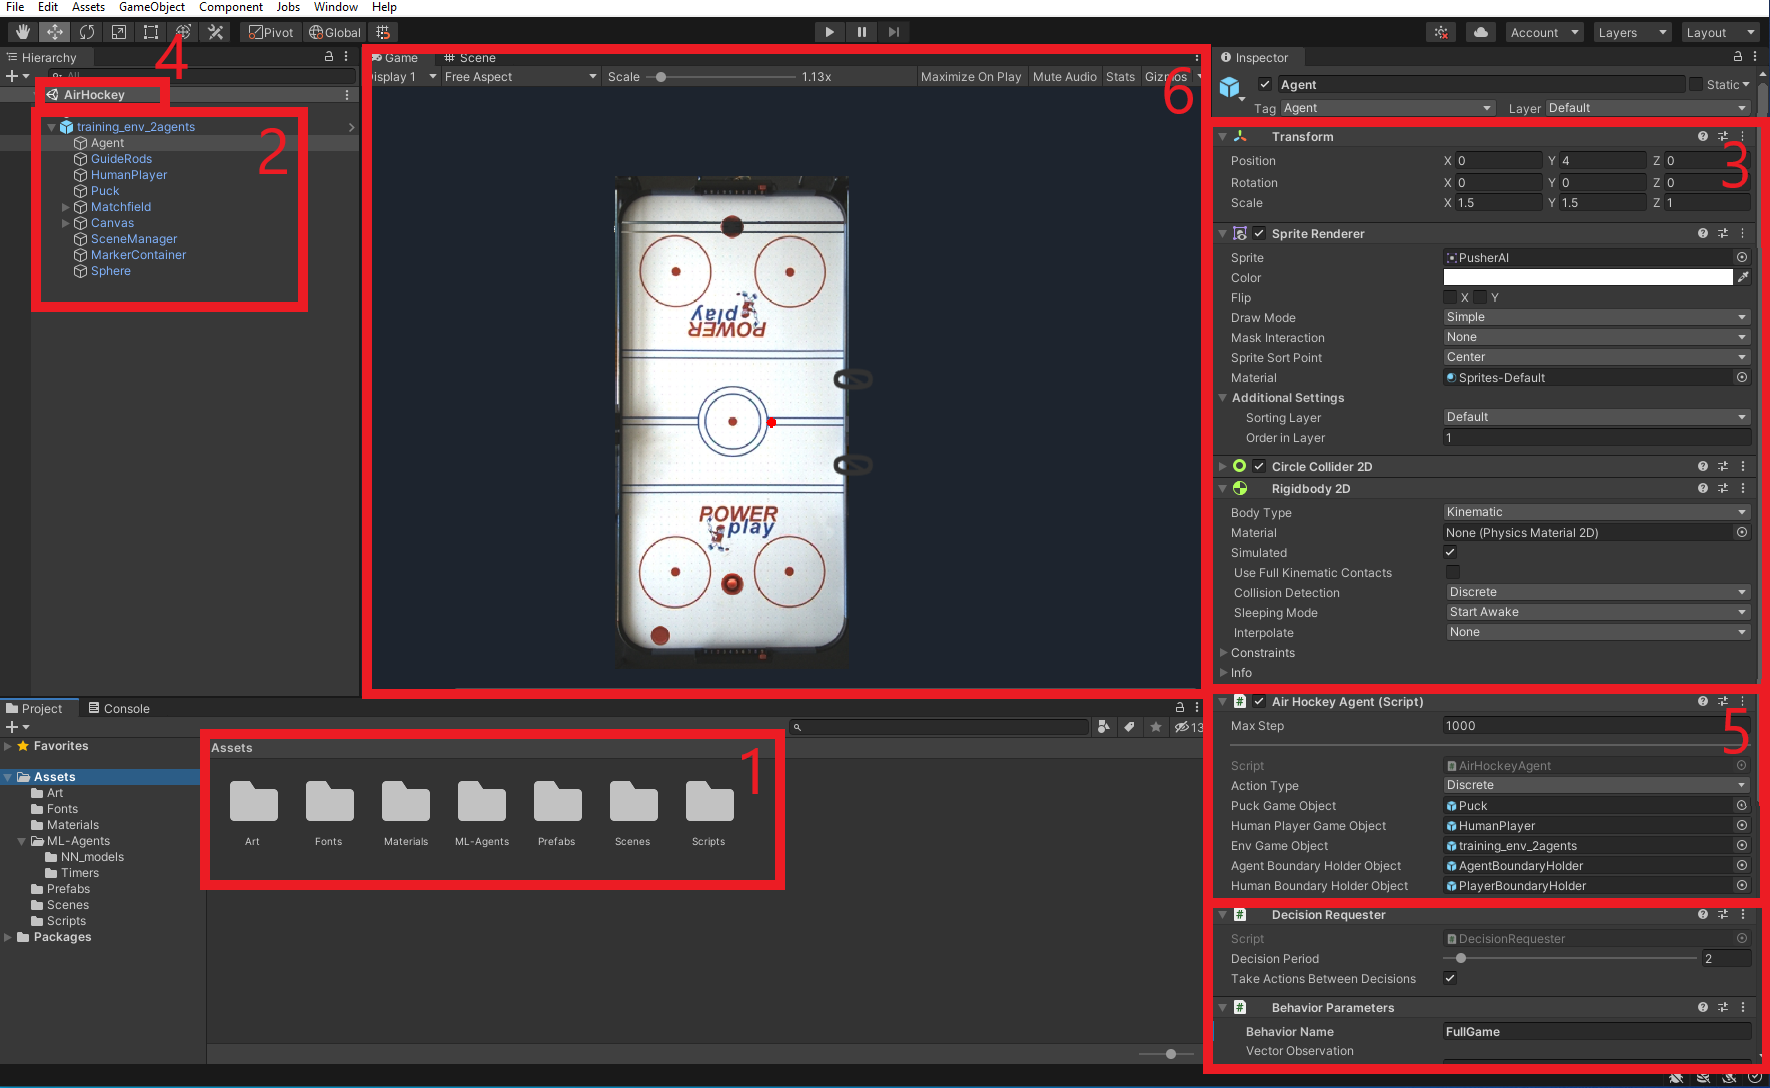
\includegraphics[scale=0.3]{images/unity_interface_marked}
\label{unity_interface_pic}
\caption{Benutzeroberfläche von Unity mit Markierungen}
\end{figure}

\begin{itemize}
\item \underline{Assets (1)} \\
Assets beinhaltet Diverses. Neben Grafiken, vorgefertigten Materialien und Szenen sind hier auch die Skripte zu finden.

\item \underline{GameObjects (2)} \\
GameObjects sind das zentrale Element von Unity. Jedes Objekt, jede Kamera und jede Grafik ist durch ein GameObject definiert. Die Funktionalitäten eines GameObjects werden durch die Components hinzugefügt. Die GameObjects sind in einem Hierarchiebaum in der Scene eingeordnet.

\item \underline{Components (3)} \\
Components geben den GameObjects ihre Funktionalität. Ein GameObject kann mehrere Components haben. Beispiele für Components sind Transform (zuständig für die Position), Collider(zuständig für die Interaktion in der Physiksimulation) und auch Skript.

\item \underline{Scene (4)} \\
Eine Scene (Szene) besteht aus GameObjects. Es ist im Prinzip die Wurzel des Hierarchiebaums. Zur Spieleentwicklung könnten hier unterschiedliche Level als unterschiedliche Scenes interpretiert werden. In unserem Fall sind nur zwei Scenes vorhanden: Eine mit einem Spielfeld zum selbst spielen und testen und eine mit acht Feldern für ein beschleunigtes Training.

\item \underline{Script (5)} :\\
Scripts sind auch Components. Sie bieten die Möglichkeit, das Verhalten selbst zu definieren. Es kann sich in Scripts auf GameObjects bezogen werden. Mit dieser Hilfe können Parameter wie das Material oder die Position geändert werden. Objekte können auch entfernt oder eingefügt werden.

\item \underline{Visualisation (6)} :\\
In diesem Bereich kann sowohl das Bild einer Kamera und  damit die Ansicht im Spiel beobachtet werden als auch eine Darstellung aller GameObjects in der Scene. Objekte können hier auch verschoben oder gedreht werden.
\end{itemize}

\subsection{Airhockey Projekt}
\label{subsect:Airhockey Projekt}

In diesem Unterkapitel werden die einzelnen GameObjects und die wichtigsten Components im Projekt vorgestellt und erklärt. Ziel ist es dabei nicht auf jedes Detail einzugehen, sondern die Arbeit für Folgeprojekte zu erleichtern. Rein optische Aspekte, wie zum Beispiel die Anzeige des Spielstandes, werden nicht betrachtet. Außerdem wird nur auf die Scene mit einem Feld eingegangen, dann die Anpassungen, die zum Kopieren gemacht werden müssen, sind nicht maßgeblich. Die folgenden GameObjects sind auch in der Abbildung \ref{unity_interface_pic} zu finden.\\

\underline{Agent} :

\begin{figure} [h]

\begin{minipage}[t]{0.6\textwidth}
\vspace{0pt}
Der Agent ist eines der zentralen GameObjects. Er hat eine Sprite Renderer Component. Dadurch kann er mit einer .png Datei visualisiert werden. Der Agent ist also ein Objekt, das im Spiel zu sehen ist. Auf der rechten Seite ist die Ansicht, wie sie auch im Projekt zu sehen ist, dargestellt.
\end{minipage}
\hspace{0.1\textwidth}
\begin{minipage}[t]{0.2\textwidth}
\vspace{0pt}

\includegraphics[width=\textwidth]{images/agent_unity}
 \caption{Ansicht des Agenten in Unity}
 \label{unity_agent}
\end{minipage}
\end{figure}

Das Agent GameObject enthält auch eine Circle Colider Component. Mit der Rigidbody Component zusammen wird die Phsyik (Reibung, Bewegung, Kollision) simuliert.\\
Ein weiterer Component des Agent Objekts ist das Script Airhockey Agent. Die Funktion von diesem Script ist die Interaktion mit der ML-Agents Toolbox. Es werden sowohl die anfallenden Rewards entsprechend des Spielverlaufes an das Netzwerk zurückgegeben, als auch die Actions entgegengenommen und damit die Umgebung (Bewegung des Agenten) beeinflusst. Zu Episodenbeginn werden in diesem Script auch die Positionen von Agent und Spieler (Pusher) zurückgesetzt. \\
Des Weiteren beinhaltet das Agent GameObject auch noch eine Decision Requester Component. Mit ihrer Hilfe wird regelmäßig ,entsprechend des Parameters Decision Periode, eine Action vom Netzwerk angefordert. Die Behavior Parameter Componente ist, neben Decision Requester, zur Parametrisierung der Nutzung des ML-Agents Toolkits nötig. Hier kann die Dimension sowohl des Actionspaces als auch die der Observation festgelegt werden. Auch Angaben zur Inferenz können hier gemacht werden. \\


\underline{HumanPlayer} :

\begin{figure} [h]

\begin{minipage}[t]{0.6\textwidth}
\vspace{0pt}
HumanPlayer ist das GameObject des zweiten Spielers. Es hat auch eine Sprite Renderer Component. Die Visualisierung ist rechts zu sehen. Da dieses Objekt auch am Spiel teilnimmt, hat es auch die Components Circle Collider und Rigidbody.
\end{minipage}
\hspace{0.1\textwidth}
\begin{minipage}[t]{0.2\textwidth}
\vspace{0pt}
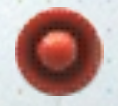
\includegraphics[width=\textwidth]{images/pusher_unity}
 \caption{Ansicht des Pushers in Unity}
 \label{unity_pusher}
\end{minipage}
\end{figure}

HumanPlayer hat auch die Components Decission Requester und Behavior Parameters. Damit wird das Selfplay ermöglicht. In unserer Implementierung wird die Version des Agenten, die den HumanPlayer bewegt nicht trainiert. Das ML-Agents Toolkit wird hier nur zur Inferenz genutzt. \\
Das Objekt enthält auch ein Script. Im Gegensatz zum Airhockey Agents Script werden hier aber keine Rewards zurückgegeben, sondern nur die Observations und die Actions behandelt. Das reicht auch aus, denn dieser Agent soll ja nicht ständig mittrainieren, sondern nur das Selfplay ermöglichen. Wenn er zu schwach wird, wird einfach die stärkere Version vom Agenten übertragen. Im Script ist auch die Option, den HumanPlayer selbst zu steuern, implementiert. Entweder mit der Tastatur oder mit einem Controller kann so der Agent in der Simulation herausgefordert werden. \\

\underline{Puck} :

\begin{figure} [h]

\begin{minipage}[t]{0.6\textwidth}
\vspace{0pt}
Der Puck ist auch ein Objekt, das wie auch der HumanPlayer und der Agent am Spiel teilnimmt. Deshalb hat es auch die Components Circle Collide und Rigidbody.  Die Components, die für das ML-Agents Toolkit nötig sind, werden hier aber nicht verwendet. Trotzdem gibt es auch hier ein c\# Script, das das Verhalten des Pucks bestimmt.
\end{minipage}
\hspace{0.1\textwidth}
\begin{minipage}[t]{0.2\textwidth}
\vspace{0pt}
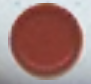
\includegraphics[width=\textwidth]{images/puck_unity}
 \caption{Ansicht des Pucks in Unity}
 \label{unity_puck}
\end{minipage}
\end{figure}
Abhängig vom Spielszenario werden in diesem Script die Startposition und die Startgeschwindigkeit des Pucks festgelegt. Auch der Spielstand wird hier mitgezählt. Die Circle Collider Componente  des Pucks erlaubt es, ein Event bei Kollision mit anderen Objekten auszulösen. Wenn der Spielfeldrand am Tor des Agenten getroffen wird, kann das mithilfe eines GameObjects ohne Renderer erkannt werden. Es kann mit einer Box Collider Componente ein Event ausgelöst werden, das den Spielstand anpasst. Das gleiche System wird auch auf der anderen Seite angewendet. \\

\underline{Matchfield} :

\begin{figure} [h]

\begin{minipage}[t]{0.6\textwidth}
\vspace{0pt}
Das GameObject Matchfield hat selbst nur eine Sprite Renderer Component, die ein Bild des Airhockeytisches zeigt. Jedoch sind diesem Objekt hierarchisch Weitere untergeordnet. Diese untergeordneten Objekte sind aber alle ohne Renderer Component und deshalb in der Spielansicht unsichtbar. Sie sind nur wegen ihrer Position interessant. Sie dienen dazu, das Spielfeld in Zonen einzuteilen. Die zulässigen Positionen von Agent, HumanPlayer und Puck werden damit auf das Spielfeld oder die jeweilige Hälfte limitiert. Die GameObjects, die zum Torezählen genutzt werden, sind auch Childobjects (hierarchisch untergeordnete Objekte) des Matchfields.
\end{minipage}
\hspace{0.1\textwidth}
\begin{minipage}[t]{0.2\textwidth}
\vspace{0pt}
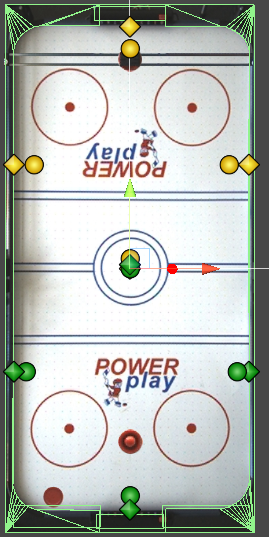
\includegraphics[width=\textwidth]{images/matchfield}
 \caption{Spielfeldbegrenzungen in Unity}
 \label{unity_matchfield}
\end{minipage}
\end{figure}
Das Matchfield hat kein Script, es wird sich nur von anderen Scripts auf die GameObjects von Matchfield bezogen. Die Transform Component, die die Position eines Objects angibt, wird dabei ausgelesen. Mit vier Objekten lässt sich damit ein rechteckiger Bereich festlegen. \\

\underline{training\_env\_2agents} :\\
Diesem Objekt sind, abgesehen von der Kamera, alle anderen GameObjects untergeordnet. Es dient als Container für das ganze Spiel. Das Objekt dient hauptsächlich zwei Zwecken:
\begin{itemize}
\item Das ganze Spielfeld kann einfacher kopiert und verschoben werden. Die Positionen der Childobjects bleiben beim Verschieben des übergeordneten Objekts relativ zu diesem unverändert. Felder könne dadurch schnell über und nebeneinander kopiert werden.
\item Das envScript ist in diesem GameObject ein Component. In diesem Script werden alle Rewards festgelegt. Auch der Spielmodus wird hier ausgewählt. Näheres zu den Rewards und den Spielmodi wir im Kapitel \ref{subsect:Airhockey Projekt} erläutert.
\end{itemize}
\chapter{Rewards und Training}  
\label{ch:rewards_training}
In diesem Kapitel wird auf das Training eingegangen. Hierbei werden die unterschiedlichen Rewards erklärt, die genutzten Netzwerke, die Hyperparameter und die einzelnen Schritte im Training. Dazu wird auch das envScript aus Unterkapitel \ref{subsect:Airhockey Projekt} noch mal genauer beleuchtet.

\section{Rewards und Umgebungsparameter}
\label{sect:rewards_params}
Hier sollen als erstes alle implementierten Rewards vorgestellt werden, damit in den folgenden Teilen der Beschreibungen des Trainings klar ist, welche Effekte sie bedingen.

\begin{itemize}
\item \underline{taskType} \\
Legt fest, welcher Spielmodus gewählt wird. Siehe dazu Abschnitt \ref{sect:spielmodi}.

\item \underline{V\_max\_puck} \\
Legt die Maximalgeschwindigkeit des Pucks fest. Einheit ist dabei nicht m/s, der Tisch ist in der Realität kleiner als in Unity. Die Ermittlung der Maximalgeschwindigkeit kann im Abschnitt \ref{sect:geschwindigkeitsmessungen} nachvollzogen werden.

\item \underline{V\_max\_robo} \\
Legt die Maximalgeschwindigkeit des Roboters fest. Messungen erfolgten analog zu denen der Maximalgeschwindigkeit des Pucks.

\item \underline{V\_max\_human} \\
Legt die Maximalgeschwindigkeit des HumanPlayer fest. Messungen erfolgten analog zu denen der Maximalgeschwindigkeit des Pucks.

\item \underline{neghumanGoalReward} \\
Dieser Reward wird vergeben, wenn der Puck in das Tor des Agenten trifft. Da es ein Gegentor ist, sollte der Reward negativ gewählt werden.

\item \underline{agentGoalReward} \\
Dieser Reward wird vergeben, wenn der Puck in das Tor des HumanPlayer trifft. 

\item \underline{avoidBoundaries} \\
Dieser Reward wird vergeben, wenn der Roboter die Bande berührt. Er sollte negativ sein. 

\item \underline{avoidDirectonChanges} \\
Dieser Reward wird vergeben, wenn der Roboter die Bewegungsrichtung ändert. Er sollte negativ sein. Der Betrag wird mit dem Betrag der Bewegungsänderung im letzten Zeitschritt multipliziert. Da dieser Reward in jedem Zeitschritt vergeben werden kann, sollte dieser Reward betragsmäßig sehr klein gewählt werden.

\item \underline{stayCenteredReward} \\
Dieser Reward belohnt den Agenten, wenn er weder links noch rechts am Spielfeldrand platziert ist. Damit kann das Verteidigungsverhalten verbessert werden. Der Reward wird zu jedem Zeitschritt vergeben und sollte deshalb sehr niedrig gewählt werden. Der Reward sinkt proportional mit der Distanz des Pushers vom Rand.

\item \underline{negoffCentereReward} \\
Dieser Reward ist vergleichbar mit dem stayCenteredReward. Jedoch ist dieser negativ zu wählen, denn er fällt betragsmäßig am höchsten aus, wenn der Agent an der Bande steht (links oder rechts).

\item \underline{encouragePuckMovement} \\
Dieser Reward belohnt die Puckbewegungsgeschwindigkeit. Er wird zu jedem Zeitschritt vergeben und sollte deshalb klein sein. 

\item \underline{encouragePuckContact} \\
Dieser Reward belohnt Kontakte mit dem Puck. 

\item \underline{contacthalf} \\
Dieser Parameter ist kein Reward sondern eine Booleanvariable. Wird sie zu True gesetzt hat das zur Folge, dass der Reward encouragePuckContact jedes mal, wenn er vergeben wird, halbiert wird. Damit wird verhindert, dass der Roboter alleine spielt oder den Puck einklemmt um den encouragePuckContact Reward auszunutzen.

\item \underline{playForwardReward} \\
Dieser Reward wird vergeben, wenn der Puck von hinten getroffen wird, also in Richtung gegnerisches Hälfte geschossen wird.

\item \underline{negplaybackReward} \\
Dieser Reward wird vergeben, wenn der Puck von vorne getroffen wird, also in die falsche Richtung geschossen wird. Er sollte negativ gewählt werden.

\item \underline{negStepReward} \\
Dieser Reward wird in jedem Fall zu jedem Zeitschritt vergeben. Er soll ein mögliches Zeitspiel des Agenten verhindern. Dazu muss er negativ sein. 

\item \underline{negMaxStepReward} \\
Dieser Reward wird vergeben, wenn die Maximallänge einer Episode erreicht wird und das Spiel deshalb abgebrochen werden muss (wird nur im Training abgebrochen, nicht im Spiel). Er sollte negativ sein.

\item \underline{behindPuckReward} \\
Dieser Reward wird zu jedem Zeitschritt, zu dem sich der Agent näher am eigenen Tor befindet als der Puck gegeben. Er sollte niedrig gewählt werden, da diese Rewardvergabe in jedem Zeitschritt möglich ist.

\item \underline{behindPuckReward} \\
Dieser Reward ist exklusiv für das Training des Spielmodus Defending. Er wird jedes Mal vergeben, wenn ein Schuss erfolgreich verteidigt wurde.

\end{itemize}

\section{Spielmodi}
\label{sect:spielmodi}
In diesem Abschnitt werden die implementierten Spielmodi beschrieben. Mit ihrer Hilfe kann die Eignung eines Netzwerk oft schneller festgestellt werden, als mit einem ganzen Spiel, da die anderen Spielsituationen nicht so komplex sind. Ein weiterer Vorteil von einfacheren Spielszenarien ist, dass damit der Agent Stufe für Stufe trainiert werden kann.

\begin{itemize}
\item \underline{Reaching} \\
Das Ziel in diesem Spielmodus ist es, den Puck zu erreichen. Dazu wird der Puck zu Beginn der Episode an einem zufälligen Ort auf der Spielfeldseite des Agenten platziert. Da HumanPlayer bei diesem Szenario keine Rolle spielt wird seine Bewegung gestoppt. Die Episode endet mit der Kollision von Agent und Puck oder beim Erreichen der maximalen Simulationsschritten. Damit ist dieser Modus von sehr niedriger Komplexität und auch für einen untrainierten Agenten schnell erlernbar.

\item \underline{Scoring} \\
Im Scoring Modus geht es nur ums Zielen und darum, das Tor zu treffen. Hier wird die Episode nicht beendet, wenn der Puck getroffen wurde, sondern wenn der Puck entweder ein Tor erreicht oder die Bande trifft. Wie beim Reaching steht der HumanPlayer unbeweglich neben seinem Tor. Da mit einem diskreten Actionspace gearbeitet wird, ist dieser Modus nicht viel verwendet worden. Wegen des diskreten Actionspace kann der Agent sich nicht präzise genug platzieren, um zu zielen. Sollte in einem Folgeprojekt jedoch mit einem kontinuierlichen Actionspace gearbeitet werden, kann dieser Modus wieder interessant werden.

\item \underline{Defending} \\
Hier hat der Agent das Ziel, sein Tor zu verteidigen. Auch in diesem Modus spielt der HumanPlayer keine Rolle. Er steht dabei unbeweglich neben seinem Tor. Der Agent wird zu Beginn der Episode an eine zufällige Position auf seiner Spielfeldseite platziert. Defending ist der einzige Modus, bei dem der Puck nicht ohne Geschwindigkeit auf das Feld gesetzt wird. Der Puck wird hier von der Seite des HumanPlayer aus mit einem zufälligen Bewegungswinkel zwischen $70^\circ$ und $-70^\circ$ auf die Seite des Agenten geschossen. Auch die Startposition variiert zufällig.Beendet wird die Episode, wenn entweder ein Tor kassiert wurde oder der Ball abgewehrt wurde. Das ist der Fall, wenn die X-Komponente der Geschwindigkeit des Pucks negativ wird, sich der Puck also auf die Hälfte des HumanPlayer zurückbewegt. In diesem Modus ist ein schneller Lernfortschritt nur mit dem defenceReward zu erwarten (bei fast allen Netzwerken).

\item \underline{FullGame} \\
FullGame ist selbsterklärend. Der Puck wird an einer zufälligen Position auf dem ganzen Spielfeld ins Spiel gebracht. Die Kontrahenten Agent und HumanPlayer werden auf ihre jeweilige Seite gesetzt und beiden ist die Bewegung im Rahmen der Parameter in envScript erlaubt. Beendet wird die Episode nur, wenn ein Tor erzielt wird oder die maximale Anzahl an Simulationsschritten erreicht wird. Diesen Modus zu meistern ist das Ziel der Trainings und eine Teilaufgabe des Projekts. Er ist zu komplex, um einen untrainierten Agenten ohne das stufenweise Ändern von Rewards zu trainieren
\end{itemize}

\begin{figure} [h]
\begin{tabular}[h]{c|c|c|c|c}
 Modus & Reaching & Scoring & Defending & FullGame \\
\hline
Puck  & Agent Seite & Agent Seite & Schuss auf Tor & Ganzes Feld \\
\hline
Agent & Agent Seite  & Agent Seite & Agent Seite & Agent Seite \\
\hline
HumanPlayer & neben Tor  & neben Tor & neben Tor & Agent Seite \\
\hline
Episodenende  & Puckkontakt & Tor, Bande & Tor verteidigt & Tor \\
 
\end{tabular}
\caption{Übersicht über die Spielmodi }
\label{modi_uebersicht}
\end{figure}

\section{Trainingsstrategie und Zwischenergebnisse}
\label{sect:trainings_strats}

In diesem Abschnitt wird das Vorgehen beim Training beschrieben und die Ergebnisse des Trainings in der Unity Umgebung gezeigt. Um die Ergebnisse einordnen zu können, werden sowohl mit Graphen der kumulativen Rewards über eine Episode als auch mit den Ergebnissen aus Spielen von Agenten untereinander gearbeitet. Zusätzlich wird eine Einschätzung der Ästethik des Spiels betrachtet.\\

\subsection{Stufenplan}
\label{subsect:stufenplan}
Da das Spiel im FullGame Modus sehr komplex ist und viele Sachen zu beachten sind, was sich auch an der Vielzahl an sinnvollen Rewards widerspiegelt, muss der Agent einige Vortrainings abschließen, um so Eigenschaften nacheinander zu erlernen. Dazu haben wir uns einen Stufenplan, der in der Abbildung \ref{training_plan} zu sehen ist, erarbeitet.

\begin{figure} [h]
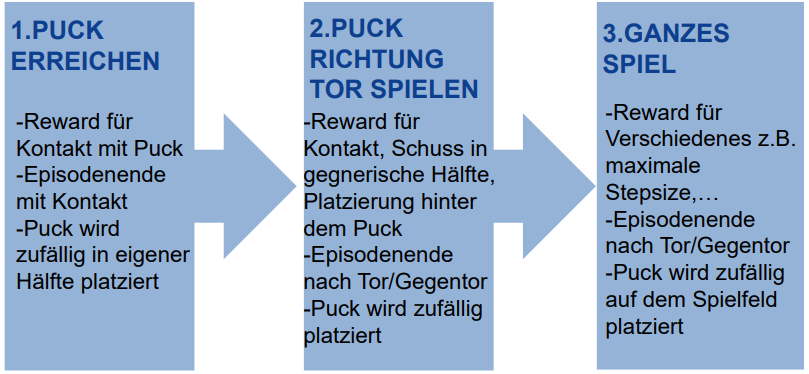
\includegraphics[scale=0.6]{images/training_strats}
\label{training_plan}
\caption{Stufenplan des Trainings}
\end{figure}

\begin{itemize}
\item \underline{1. Puck erreichen} \\
Der erste Lernschritt des Agenten ist es, den Puck zu erreichen. Diese Fähigkeit kann im Reaching Modus schnell mit effektiv nur einem Reward (encouragePuckContact) erlernt werden. Ein Nachteil beim Üben im Reaching Modus ist, dass bewegte Ziele nicht vorkommen und somit diese auch noch nicht trainiert werden können.

\item \underline{2. Puck richtung Tor spielen} \\
Bei diesem Schritt wird auf dem vortrainierten Agenten aufgebaut. Das Ziel ist es hier den Puck in Richtung des gegnerischen Tors zu spielen. Es macht Sinn, diese Fähigkeit zuerst im Reaching Modus zu üben und erst danach in den FullGame Modus zu wechseln. Dadurch ist der Anstieg an Komplexität geringer. Hier werden die Rewards playForwardReward und negplaybackReward als Hauptrewards genutzt. Es hat sich jedoch gezeigt, dass die Rewards encouragePuckContact und behindPuckReward hier auch nützlich sind. Dadurch wird verhindert, dass der Agent, falls er vor dem Puck erscheint, die ganze Episode abwartet, um den negplaybackReward zu verhindern. Mit einem ähnlichen Satz an Rewards kann dann auch im FullGame Modus das Training fortgesetzt werden. Die Stärke des Gegners spielt dabei keine große Rolle, da keine negativen Rewards für Gegentore gegeben werden.

\item \underline{3. Ganzes Spiel} \\
Diese Stufe im Plan ist mit Abstand die Zeit intensivste. Da hier das erste mal Rewards und Bestrafungen für  Tore genutzt werden, ist die Wahl des Gegners nun ein sehr wichtiges Thema. Ist der Gegner zu schwach, kann nicht viel gelernt werden. Ist der Gegner zu stark, wird der Agent schnell passiv und versucht das Spiel auszubremsen um ein Gegentor zu verhindern. Bei diesem Schritt ist also die Balance zwischen der Anregung zum Spiel durch Rewards, wie negStepReward und encouragePuckMovement, und der Herausforderung durch den Gegner nicht einfach zu schaffen. Hinzu kommt, dass einige Reward Konstellationen zu unerwünschtem Verhalten führen. Ist beispielsweise der behindPuckReward hoch, der Gegner stark (in Vergleich zum Agenten) und der neghumanGoalReward hoch, neigt der Agent schnell dazu, sich nahe ans eigene Tor zu stellen und das Ende der Episode abzuwarten. Ist der Reward avoidDirectionChanges hoch, kann es passieren, dass der Roboter dazu neigt, oft bis an den Rand zu fahren. Der stayCenteredReward kann hier entgegenwirken. \\ 
Dadurch, dass oft unvorhergesehenes schlechtes Verhalten erlernt wird, ist es wichtig, den vorherigen Stand des Agenten zu sichern und gegebenenfalls den Fortschritt zu verwerfen, weil dieser eher einem Rückschritt gleicht. Dann kann mit einem neuen Reward- oder Parametersatz oder mit einem anderen Gegner ein weiterer Versuch vom gesicherten Stand aus probiert werden. 
\end{itemize}

\subsection{Netzwerkauswahl und Zwischenergebnisse}
\label{subsect:netzwahl_ergs}

In diesem Abschnitt sollen die Ergebnisse von zwei Netzwerken und ihren Hyperparametern verglichen werden. In diesem Stil wurden noch andere Konstellationen von Hyperparemetern verglichen. Nach Abwägung der Trainingsgeschwindigkeit gegen die Komplexität, wurde sich dann für die Parametersätze, welche in den Konfigurationsdateien zu finden sind, entschieden. \\
Das ML-Agents Toolkit stellt sowohl PPO als auch SAC Agenten zur Verfügung. Um nicht unnötige Ressourcen zu verschwenden, macht es jedoch keinen Sinn, zwei unterschiedliche Agenten zu trainieren. Deshalb wurde hier entschieden, sowohl einen PPO als auch einen SAC Agenten, jeweils das gleiche Einstiegstraining durchlaufen zu lassen. Anhand der Leistung dabei wurde dann die Wahl entschieden, mit welchem Netzwerk das weitere Training stattfinden soll. \\

Das Einstiegstraining erfolgte für beide Agenten mit genau den gleichen Rewards, in der gleichen Umgebung und mit den gleichen Parametern. Es beinhaltet insgesamt fünf Einzeltrainings, nach denen Rewards oder Parameter angepasst wurden. 

\begin{itemize}
\item 1: Im Reaching Modus wird nur mit dem encoragePuckContact Reward das Netzwerk für 500k (500 000) Episoden trainiert. 

\item 2: Das zweite Training erfolgt immer noch im Reaching Modus, jedoch wird der encouragePuckContact Reward reduziert und der playForwardReward dazugenommen. Auch ein kleiner negStepReward wird genutzt. Das Training endet nach 1M (1 000 000) Episoden.

\item 3: Dieses Training erfolgt nun im FullGame Modus. Neben den Rewards für Tore werden hier einige andere Rewards hinzu genommen um das Spielverhalten zu formen. Als Gegner wird ein anderer PPO Agent verwendet, der vorher schon etwas besser trainiert wurde. Dessen Geschwindigkeit wird aber stark limitiert um das Spiel fair zu halten. Es wird so für weitere 1M Episoden trainiert.

\item 4: Nach dem letzten genannten Trainingsschritt ist aufgefallen, dass sich der Agent oft weit am Spielfeldrand befindet und so die Verteidigung vernachlässigt. Deshalb wurden für dieses Training die Rewards angepasst. Auch die Geschwindigkeit des HumanPlayers wurde erhöht, um dem Agenten besser gewachsen zu sein. So wurde dann bis insgesamt 3M Episoden trainiert.

\item 5: Dieses Training unterscheidet sich nicht vom Vierten. Mit den gleichen Voraussetzungen wurde das Training bis 4M fortgesetzt
\end{itemize}

Die Ergebnisse dieser Trainings sind im Folgenden dargestellt. In den Abbildungen sind jeweils die Graphen des PPO-Agenten und des SAC-Agenten übereinandergelegt. Der linke Graph zeigt dabei die Entwicklung des kumulativen Rewards über die Anzahl der verstrichenen Trainingsepisoden, der rechte die Entwicklung der Episodenlänge. Da die Trainings aufeinander aufbauen, sind in den Graphen der fortgeschrittenen Trainings die  Vorangegangenen auch enthalten.\\
\newpage
\begin{figure} [h]
\underline{1. Training bis 500k} \\

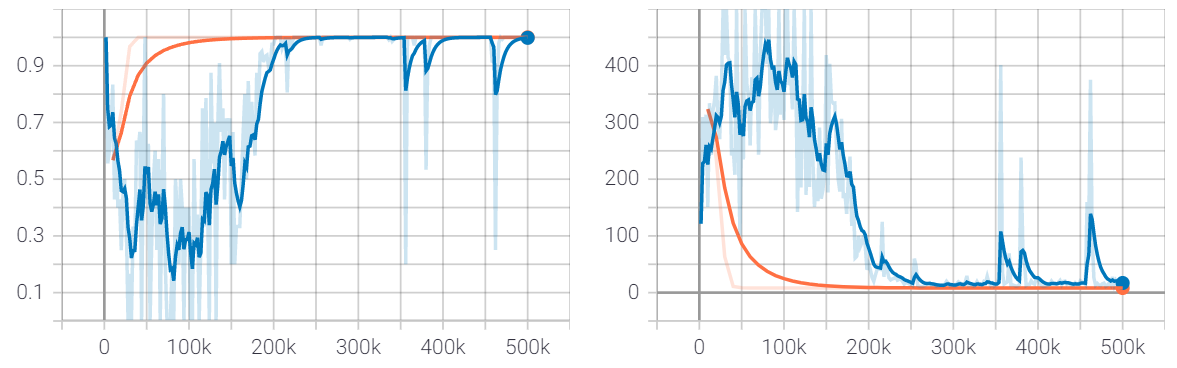
\includegraphics[width=\textwidth]{images/reaching_erg}
\caption{Orange: PPO-Agent, Blau: SAC-Agent}
Der maximal erreichbare kumulative Reward ist in dieser Trainingsphase 1. Am Graph ist zwar zu erkennen, dass der PPO-Agent dieses Ergebnis schneller und ohne Ausreißer erreicht, aber der SAC-Agent erreicht das Ziel auch. Beobachtet man die beiden Agenten in der Unity-Umgebung bei der Aufgabe, sind sie vom Verhalten her praktisch nicht zu unterscheiden. Beide bewegen sich auf sehr kurzem Weg auf den Puck zu.
\end{figure}

\begin{figure} [h]
\underline{2. Training bis 1M} \\
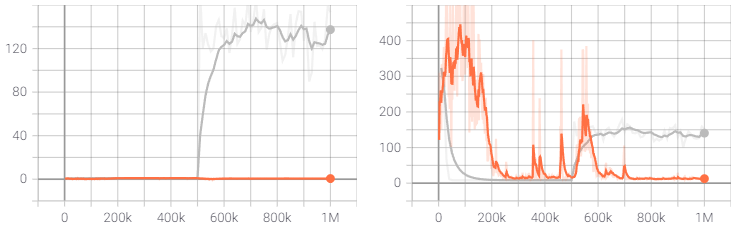
\includegraphics[width=\textwidth]{images/rea2_erg}
\caption{Grau: PPO-Agent, Orange: SAC-Agent}

In diesem Trainingsabschnitt hat der PPO-Agent nach den Rewards klar den Vorteil. Jedoch kann man an der Episodenlänge sehen, dass die Aufgabe nicht zufriedenstellend erlernt wurde. Da die Episode beim Puckkontakt beendet wird, sollten sie sehr kurz ausfallen. Beim Beobachten des Spielverhaltens ist dies auch festzustellen. Der PPO-Agent neigt dazu, in der Nähe des Pucks in einen "Zitterzustand" überzugehen, welchen schnelle Richtungsänderungen charakterisieren. Geht er nicht in diesen Zustand, trifft er den Puck aber öfter von der richtigen Seite, als von der Falschen. Auch der SAC-Agent trifft den Puck öfter von der richtigen Seite, als von der Falschen. Er zeigt aber die Verhaltensauffälligkeit mit dem Zittern nur äußerst selten und ist damit insgesamt besser, als der PPO-Agent nach diesem Training in der zugehörigen Aufgabe.
\end{figure}

\begin{figure} [h]
\underline{3. Training bis 2M} \\
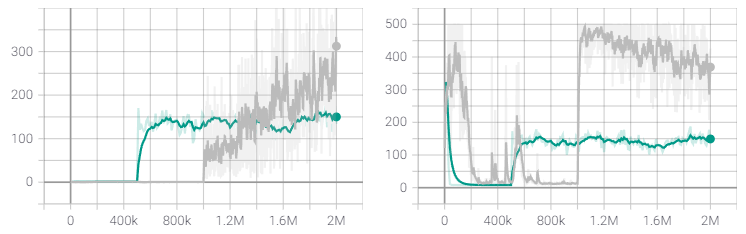
\includegraphics[width=\textwidth]{images/fullgame_erg}
\caption{Grün: PPO-Agent, Grau: SAC-Agent}
Der SAC-Agent hat in dieser Trainingsperiode seinen Rückstand in der Kategorie kumulativer Reward nicht nur verkürzt, sondern hat den PPO-Agent sogar überholt. Die Episodenlänge hat sich dabei erhöht. Da das Training im FullGame Modus erfolgte und diese Agenten jetzt dafür geeignet sein sollten, ist eine gute Möglichkeit sie zu vergleichen, das direkte Spiel gegeneinander. Hier schneidet der PPO-Agent eindeutig besser ab als der SAC-Agent. Er schlägt diesen mit 10:5. Außerdem ist sein Spielverhalten deutlich besser. Währen der SAC-Agent sich oft unkontrolliert bewegt, ohne den Puck zu spielen (höhere Episodenlänge), lässt sich bei seinem PPO-Kontrahenten deutlich erkennen, dass er nicht nur zielstrebig auf den Puck zufährt, sondern ihn meist auch in die richtige Richtung spielt.
\end{figure}

\begin{figure} [h]
\underline{4. Training bis 3M} \\
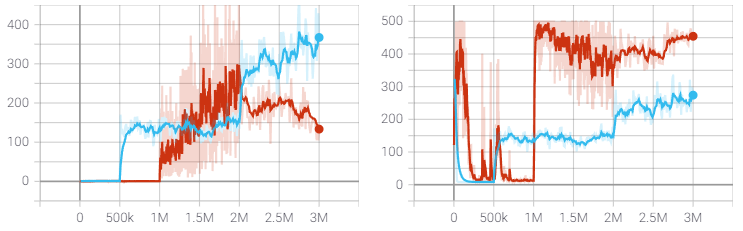
\includegraphics[width=\textwidth]{images/centered_erg}
\caption{Blau: PPO-Agent, Orange: SAC-Agent}
Bei diesem Training überholt der PPO-Agenten den SAC- Agenten in Sachen kumulativer Reward wieder. Auch beim Spielverhalten ist er ihm noch überlegen und schlägt ihn mit 10:4. Das Verhalten des SAC-Agenten hat sich selbst nach dem Training noch nicht deutlich verbessert. Er ist immer noch sehr passiv, wenn er einen Kontakt macht, ist dieser jedoch meist nicht schlecht. Insgesamt ist der SAC-Agent aber immer noch weit von einem Sieg entfernt.
\end{figure}

\begin{figure} [h]
\underline{5. Training bis 4M} \\
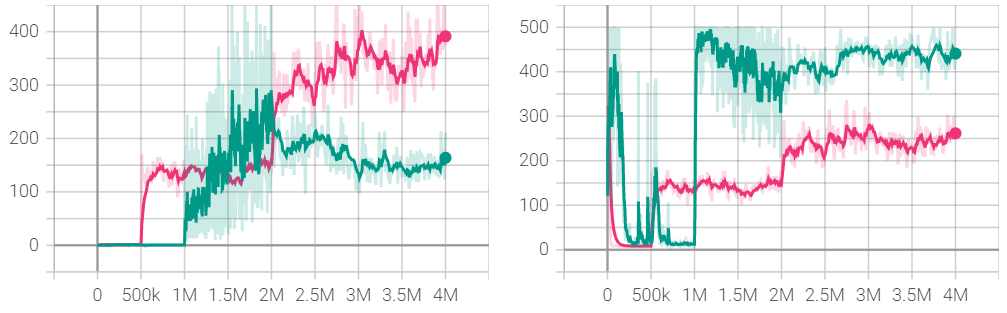
\includegraphics[width=\textwidth]{images/centered2_erg}
\caption{Rosa: PPO-Agent, Grün: SAC-Agent}
In der letzten Trainingsetappe stagnieren nicht nur die kumulativen Rewards weitgehend, sondern auch das Spielverhalten ist weitgehend unverändert. Der PPO-Agent ist dem SAC-Agenten immer noch voraus. \\
Insgesamt haben die Erfahrungen im gesamten Training gezeigt, dass der PPO-Agent gegenüber dem SAC-Agenten für diese Anwendung im Vorteil ist. Bei genau gleichem Training hat er ein weit besseres, aktiveres, intelligenter wirkendes Spielverhalten entwickelt. Zusätzlich hat es den Anschein, dass sich die Verhaltensentwicklung beim PPO-Agenten besser abschätzen lässt. Die erwünschten Verhaltensmuster sind dadurch einfacher zu erreichen. Aus diesen Gründen wurde für den größten Teil der Trainingsbemühungen mit einem PPO-Agenten, der Parametrisierung des hier verwendeten Netzwerkes gearbeitet.
\end{figure}
\begin{figure}[h]
\section{Trainingsverlauf und Ergebnis}
\label{sect:training_erg}

Der vorhergegangene Abschnitt \ref{subsect:netzwahl_ergs} hat bereits einen guten Einblick über das Vorgehen beim Training gegeben. Dieser soll noch einige Informationen zur Gegnerauswahl, zum Fortschritt, zu den Kriterien eines guten Agenten und zu den besten bereits erzielten Ergebnissen geben.

\subsection{Gegnerwahl}
\label{subsect:gegner}

Im letzten Abschnitt war zu erkennen, dass die ersten Trainings im Reaching Modus absolviert werden und deshalb dabei kein Gegenspieler benötigt wird. Diese Trainings sind jedoch ziemlich simpel und können schnell erfolgreich abgeschlossen werden. Der größte Teil des Trainings wird also mit einem Gegenspieler durchgeführt. Um zu verhindern, dass der Agent entweder nichts lernt (Gegner zu schwach) oder sich weigert, den Puck zur gegnerischen Hälfte zu spielen, weil er einen gefährlichen Schuss befürchtet (Gegner zu stark), muss ein adäquater HumanPlayer als Trainingspartner genutzt werden. Im Verlauf des Trainings bietet es sich an, die Methode des Selfplay zu nutzen. Hierbei bespielt sich der Agent selbst beziehungsweise eine Version von sich selbst. Dabei ist darauf zu achten, dass man das Netzwerk des Agenten nicht zu oft oder zu selten auf den HumanPlayer überträgt. Bei zu häufigen Transfers besteht die Gefahr, dass die Gegenspieler "zusammen spielen" und somit zum Beispiel einem Kontaktreward schnell einen Torreward obsolet machen. Um einen solchen Effekt zu erzielen, muss das Netzwerk aber oft übertragen oder gar für beide Spieler gleichermaßen trainiert werden. Bei zu geringen Transfers kann ein Training ohne vernünftige Herausforderung an Effizienz verlieren. Ein weiteres Problem des Selfplay ist, dass man zu Beginn gar keine Ergebnisse hat, welche als Gegner verwendet werden können. Deshalb ist in diesem Projekt auch ein festprogrammierter Spieler implementiert. Dieser bewegt sich stets hinter den Puck, wenn auf seine Seite gespielt wird, und spielt diesen zurück. Da die Richtung des Rückspiels aber nicht beachtet wird, ist die Gefahr eines Gegentores nicht so besonders groß. Besonders bei gedrosselter Geschwindigkeit ist er also ein idealer Einstiegsgegner.
\end{figure}
\begin{figure}[h]
\subsection{Qualitätskriterien}
\label{subsect:kriterien}
 
Um einen guten Agenten trainieren zu können, muss zunächst geklärt werden, was ein guter Agent ist. Im Gegensatz zu einem Läufer, den man nur nach einem Kriterium bewertet (seiner benötigten Zeit um eine Strecke zurückzulegen), kann ein Agent nicht so einfach objektiv bewertet werden. \\
Eine erstrebenswerte Eigenschaft ist es, dass gegen möglichst viele unterschiedliche Gegner aus möglichst vielen Spielsituationen ein Tor erzielt wird. Analog dazu ist es auch erstrebenswert, gegen möglichst viele unterschiedliche Gegner aus möglichst vielen Spielsituationen kein Gegentor zu kassieren. Auch wenn viele Spielentscheidungen beide genannten Eigenschaften gleichzeitig begünstigen, kann doch eine besonders riskante Spielweise sowohl die Wahrscheinlichkeit, ein Tor zu machen als auch die Wahrscheinlichkeit eines Gegentores erhöhen. Ist demnach ein besonders defensives oder ein offensiveres Vorgehen besser? Da der Grad der Offensivneigung jedoch schwer zu messen ist und nicht mal klar ist, ob sie erwünscht ist, wird in dieser Arbeit hauptsächlich auf die Tordifferenz der Agenten geachtet. Diese Bewertung wurde dann im Spiel gegen einen älteren Agenten durchgeführt. Um zu verhindern, dass der Agent anfällig für einen menschlichen Spieler wird, wurde seine Spielfähigkeit von Zeit zu Zeit auch von einer Person per Tastatur oder Controller validiert. Logischerweise ist es jedoch nicht möglich, gegen einen menschlichen Spieler zu trainieren. Bei diesen Testspielen hat sich herausgestellt, dass bei den fortgeschritteneren Agenten einige dabei sind, die manuell nicht mehr besiegt werden können und teilweise sehr hoch in diesen Tests gewonnen haben. Diese Niederlage der menschlichen Testspieler ist jedoch ein Zeichen für ein gutes Trainingsergebnis.\\
Neben der Fähigkeit, viele Tore zu schießen, ohne im Gegenzug viele zu kassieren, ist auch die Ästhetik der Bewegungen nicht unwichtig. Da das Ziel des Projekts ein Demonstrator ist, ist ein nachvollziehbares Spielverhalten sinnvoll. Ein weiterer Punkt ist die Lärmbelastung. Auch wenn in Unity das Zittern keinen Nachteil mit sich bringt, kommt es dadurch am realen Tisch durch die Motoren zu schrillen, unangenehmen Geräuschen. Das sollte beim Training beachtet werden.
\end{figure}


\chapter{Realer Demonstrator}  
\label{ch:realer demonstrator}
In diesem Kapitel werden die nötigen Punkte zum Übergang auf den Demonstrator angesprochen. Dazu gehören die Messungen von Maximalgeschwindigkeiten, die Bildverarbeitung, Sicherheitsvorkehrungen um Kollision und Schaden zu verhindern und ein Benutzerinterface für den Bedierner des Demonstrators. Alle Bildverarbeitungsschritte wurden in Python mit der OpenCV Bibliothek durchgeführt.

\section{Geschwindigkeitsmessungen}
\label{sect:geschwindigkeitsmessungen}

Bei den Geschwindigkeitsmessungen wurden die Maximalgeschwindigkeit von Roboter und Puck gemessen. Während die Maximalgeschwindigkeit des Roboters relativ einfach erreicht werden kann ist die des Pucks abhänig vom Spieler. Unsere Messung wurde deshalb an einem Schuss durchgeführt, denn wir nach bestem Gewissen als ausreichend schnell bewerten würden. Gemessen wurde anhand von Videomaterial der Kamera. Mit dem Programm Tracker des Open Source Physics Projekts \cite{tracker} wurde das Material analysier. Diese Software erlaubt es einen Punkt (Puck oder Roboter) von Frame zu Frame zu verfolgen. Mit der Bildwiederholungsrate und einem Maßstab können nun Werte ermittelt werden. Da diese Werte für das Training in der Softwareumgebung von Nöten ist wurde als Maßstab nicht die Abmessung in Metern des realen Demonstrators genutzt sondern die Länge in Unitylängeneinheiten. Die Ergebnisse sind wie folgt ausgefallen:\\
\begin{figure}
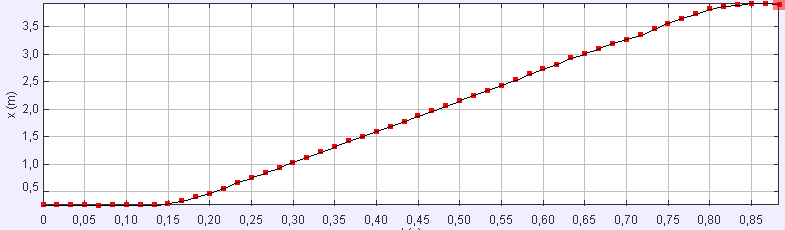
\includegraphics[width=\textwidth]{images/messung_robo_x}
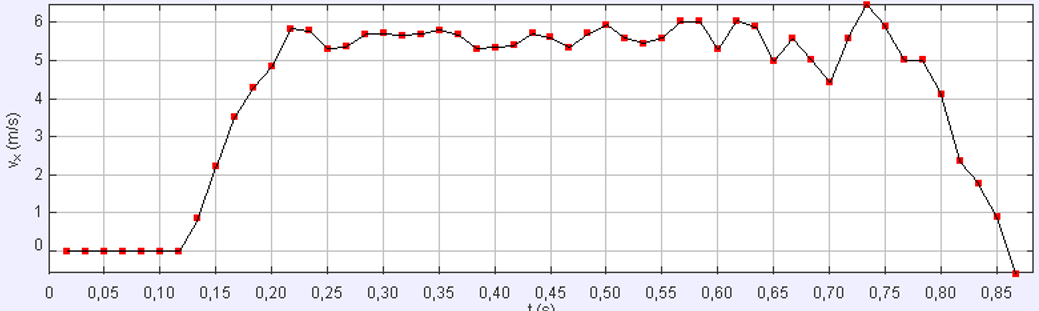
\includegraphics[width=\textwidth]{images/messung_robo_v}
 \caption{Messwerte des Roboters }
 \label{mess_robo}

Das obere Diagramm in Abbildung \ref{mess_robo} zeigt den zurückgelegten Weg des Roboters über die verstrichene Zeit seit Beginn der Messung. Das untere zeigt den Geschwindigkeitsverlauf über die Zeit. Die Maximalgeschwindigkeit ist also in etwa 6m/s. Da im Wegdiagramm in sehr guter Näherung eine Gerade während der Bewegung zu sehen ist kann die Geschwindigkeit während dieser Zeit als konstant angenommen werden. Rechnent man die Durchschnittsgeschwindigkeit über den Zeitraum von 0.2 bis 0.75 Sekunden aus so erhält man bei einem zurückgelegten Weg von 3.2 (LE)Längenenheiten eine Geschwindigkeit von 5.8 LE/s. Nach Rundung wurde mit dem Wert 6 LE/s traininiert.
\end{figure}

\begin{figure}
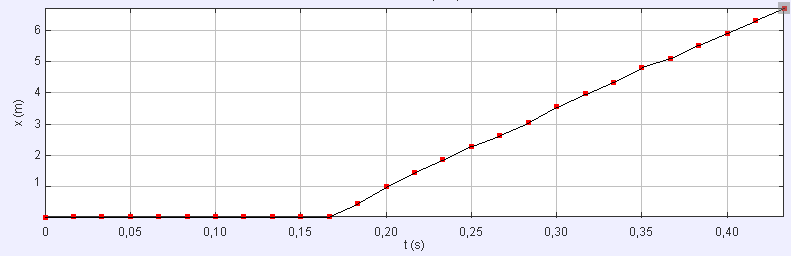
\includegraphics[width=\textwidth]{images/messung_bolzen_x}
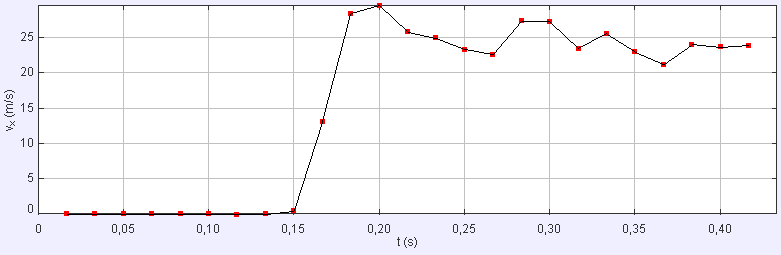
\includegraphics[width=\textwidth]{images/messung_bolzen_v}
 \caption{Messwerte des Pucks}
 \label{mess_puck}
Diese Diagramme sind von der Messung der Bewegung des Pucks. Auch hier zeigt da obere den Verlauf des zurückgelegten Weges und das untere den Geschwindigkeitserlauf über die Zeit. Rechnet man hier die Steigung der Geraden im Wegdiagramm mit einer Wegdifferenz von 6.8 LE und einer verstrichenen Zeit von 0.33 Sekunden aus, so ergibt sich ein Wert von 20.6 LE/s. Da die Puckgeschwindigkeit bei anderen Spielern noch höher sein könnte wurde für die Simulation in Unity und damit auch für die Trainings eine Maximalgeschwindigkeit des Pucks von 25 LE/s angenommen. 
\end{figure}

\clearpage
\begin{figure}
\section{Benutzeroberfläche}
\label{sect:gui}
Das graphical use interface (GUI) wurde in Python geschrieben. Die Bibliothek Tkinter wurde dabei genutzt. Diese Bibliothek wurde unter einer Pythonlizenz veröffentlicht und ist so frei für alle zugänglich. Dadurch ist der Einsatz der GUI in jedem Fall rechtlich unbedenklich.\\

\subsection{Ansicht der Oberfläche}
\label{subsect:gui_pic}


Die Folgende Abbildung zeigt das Interface. Die markierten Bereiche und Elemente werden im Folgenden erklärt.\\
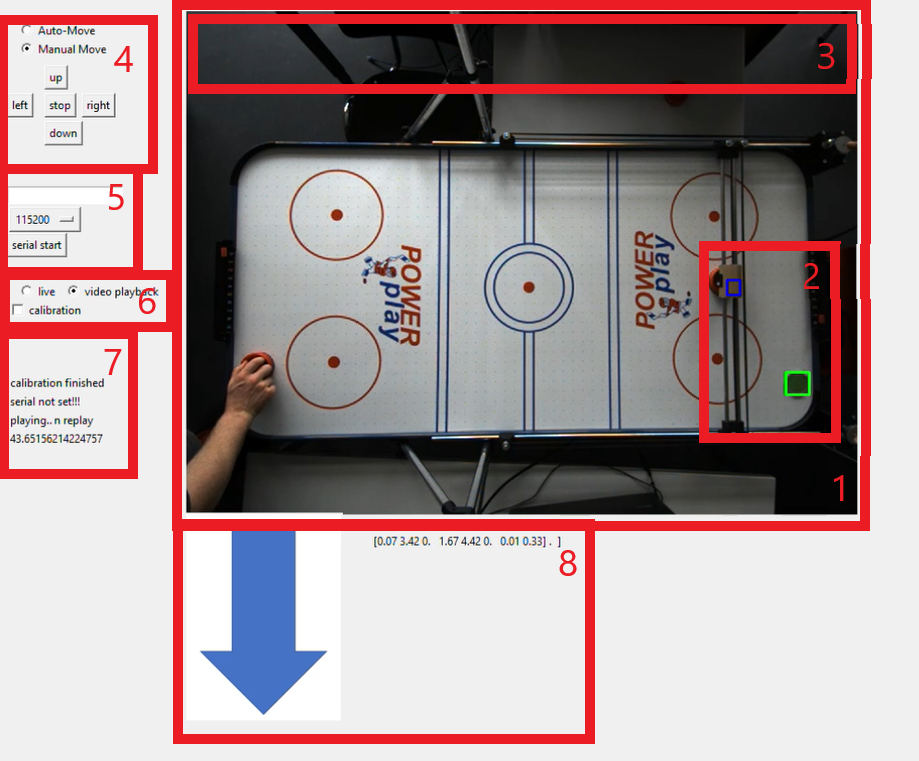
\includegraphics[width=\textwidth]{images/gui_pic_marked}
 \caption{Benutzeroberfläche}
 \label{gui_pic}

\end{figure}
\begin{figure}
1:\\
Hier ist das Kamerabild oder eine Videosequenz zu sehen. Das Bild wird wird, je nach Zustand, um einige Informationen ergänzt.\\
2:\\
Eine Ergänzung zum Kamerabild ist die Markierung von Roboter und Puck sofern sie erkannt wurden. Der Puck wird mit einem grünen und der Roboter mit einem blauen Rechteck markiert.
\\
3:\\
In diesem Bereich wird eine Meldung gegeben wenn, wenn Puck oder Robote nicht erkannt werden.\\
4:\\
In diesem Bereich sind die Bedienelemente für das manuelle Verfahren. Mit den beiden Knöpfen kann eine Auswahl zwischen einem autonomen Bewegungsmodus (Auto-Move) und dem manuellen Verfahrmodus gemacht werden. Ist der manuelle Modus ausgewählt kann mit den darunter liegenden Feldern der Roboter bewegt werden. Im Auto-Move Modus obliegt die Entscheidung sich zu bewegen dem Agenten. Der Agent kann im Gegensatz zum manuellen Modus auch diagonal verfahren. \\
5:\\
Hier kann die serielle Kommunikation gesteuert werden. Im Eingabefenste muss der Port eingegeben werden (z.B. COM4). Darunter ist ein Drop-Down Menü, in dem die Baudrate gewählt werden kann. Mit dem Knopf serial start wird die Kommunikation aufgebaut. Besteht schon eine wird die alte erst beendet bevor eine neue aufgebaut wird.\\
6:\\
Im diesem Ausschnitt kann die Videoquelle gewählt werden. Bei live wird auf das aktuelle Kamerabild zugegriffen, bei video playback kann eine Aufnahme genutzt werden. Das ist besonders nützlich wenn zuhause am Schribtisch  am Projekt gearbeitet werden muss und man unabhänig vom Zugang zum Airhockey-Tisch sein will. In der kleinen Box darunter kann der Kalibrierungsmodus initialilisiert werden. Die Box bleibt dann ausgewählt bis die  Kalibrierung erfolgreich abgeschlossen wurde.\\
7:\\
In diesem Bereich werden nur Statusmeldungen gemacht. Er enthält keine Bedienelemente. Die erste Zeile gibt Aufschluss über den Status der Kalibrierung. Die zweite informiert über die serielle Kommunikation. Die dritte enthält eine Aussage über den Spielmodus. In der letzten wird angegeben, mit welcher Frequenz die ganze Anwendung läuft.\\
8:\\
Hier sind Eingang und Ausgang des neuronalen Netzwerkes angegeben. Der Vektor enthält die Informationen zum Spielgeschehen aus der Bildverarbeitung und der Pfeil zeigt das Ergebniss der Interferenz an. 
\end{figure}
\clearpage

\subsection{Programmablauf der GUI-Anwendung}
\label{subsect:pap}

In diesem Abschnitt wird der Ablauf der einzelnen programmtechischen Schritte erklärt. Zu beachten ist dabei, dass zwei Prozess parallel ablaufen müssen. Das liegt daran, dass das Interface kontinuierlich überwacht und auf Eingaben überprüft werden muss. Gleichzeitig müssen die anderen Vorgänge zur Bildverarbeitung, zur Kommunikation etc. ablaufen. 
Der Prozess für die Funktion der Oberfläche und der Prozess für den standartmäßigen Ablauf sind also immer aktiv, beziehungsweise laufen in einer Schleife und werden koninuierlich wiederholt. Wenn eine Benutzerinteraktion ausgelöst wird, wird diese in die Schleife der  Interfacefunktion oder der Standartabläufe eingefügt. Wird beispielsweiße ein Haken in der Box zur Kalibrierung erfasst ändert das den Standartablauf, wird der Knopf für die serielle Kommunikation gedrückt verlängert das die Schleife des Interfaces. Alle Funktionen, die direkt durch ein Bedienelement hervorgerufen weden verlängern die Interfaceschleife, der Rest, bei dem nur ein Parameter angepasst wird, wird während des Standartablaufen abgearbeitet.\\
 Funktionen der Interfaceschleife sind:\\
\begin{itemize}
\item manuelle Bewegung
\item Start der seriellen Kommunikation
\item Wechsel der Videoquelle
\end{itemize}

Wie die anderen Funktionen abgearbeitet werden ist in der Abbildung \ref{gui_pap} dargestellt. Im Ablaufgraphen stelle die grünen Rechtecke Programmschritte dar. Habe die Rechtecke links und rechts einen Doppelstrich bedeutet das, dass diese Prozesse komplexer sind und noch genauer erläutert werde. Die orangenen Rauten stehen für eine Entscheidung. Die Sechsecke stellen Anfang und Ende der Schleife dar.\\\\

Zu Beginn des Programms wird die Viualisierung erstellt. Dazu wird ein Objekt der Klasse Window angelegt. Dieses hat durch Vererbung aus der Tkinter Bibliothek die nötigen Methoden und Attribute um das Fenster mit der mainloop Methode zu erstellen und die beiden Schleifen zu starten. \\
Im Standartablauf wird als erstes überprüft, ob schon eine Videoquelle festgelegt wurde. Ist das nicht der Fall, so ist der Durchlauf der Schleife schon vorbei. \\
Als nächstes wird geprüft, ob eine Kalibrierung durchgeführt werden soll. Ist das der Fall wird ein Kalibrierungsversuch unternommen. Scheitert dieser, so wird sofort zum Update des Interfacebildes gesprungen. Ist er erfolgreich so kann der Standartablauf weiter verfolgt werden.\\
Die nächste Abfrage ist, ob schon kalibriert wurde. Das ist wichtig, denn es besteht auch die Möglichkeit, dass noch nicht kalibriert wurde und der Haken im Interface noch nicht gesetzt wurde.\\
Nun erfolgt der Schritt, bei dem die Input Daten für den Agenten aus dem Kamerabild ermittelt werden.\\
Wenn Puck und Roboter erkannt werden kommt es zu Spielen. Dabei wird die Ausgabe des Netzwerkes nach einer Sicherheitsüberprüfung ausgeführt.\\
Ist es der Fall das nur der Roboter erkannt wird ist davon auszugehen, dass der Puck nicht im Spiel ist. Dann wird der Roboter in eine Ausgangsposition mittig vor dem Tor fahren und auf die Fortsetzung des Spiels warten.\\
Da es durchaus vorkommen kann, dass durch die Lichtverhältnisse oder Ähnlichen für ein oder zwei Einzelbilder nicht Puck und Roboter erkannt werden obwohl beide am Tisch sind wird in diesem Fall der letzte Bewegungsbefehl wiederholt. Dazu wird überprüft, wie lange die Berechnung des letzten Befehls zurück liegt. Ist er zu alt wird in die Ausgangsposition verfahren.\\
Wenn der Roboter zu lange nicht mehr erkannt wurde wird jede Bewegung verhindert um eine Kollision zu verhindern. Dabei ist es egal ob der Puck noch detektiert wird.\\
Als letzter Punkt der Schleife steht das Update des Bilds für das Interface. Das erfolgt immer, außer es gibt keine Videoquelle.\\ 




\begin{figure}[h]
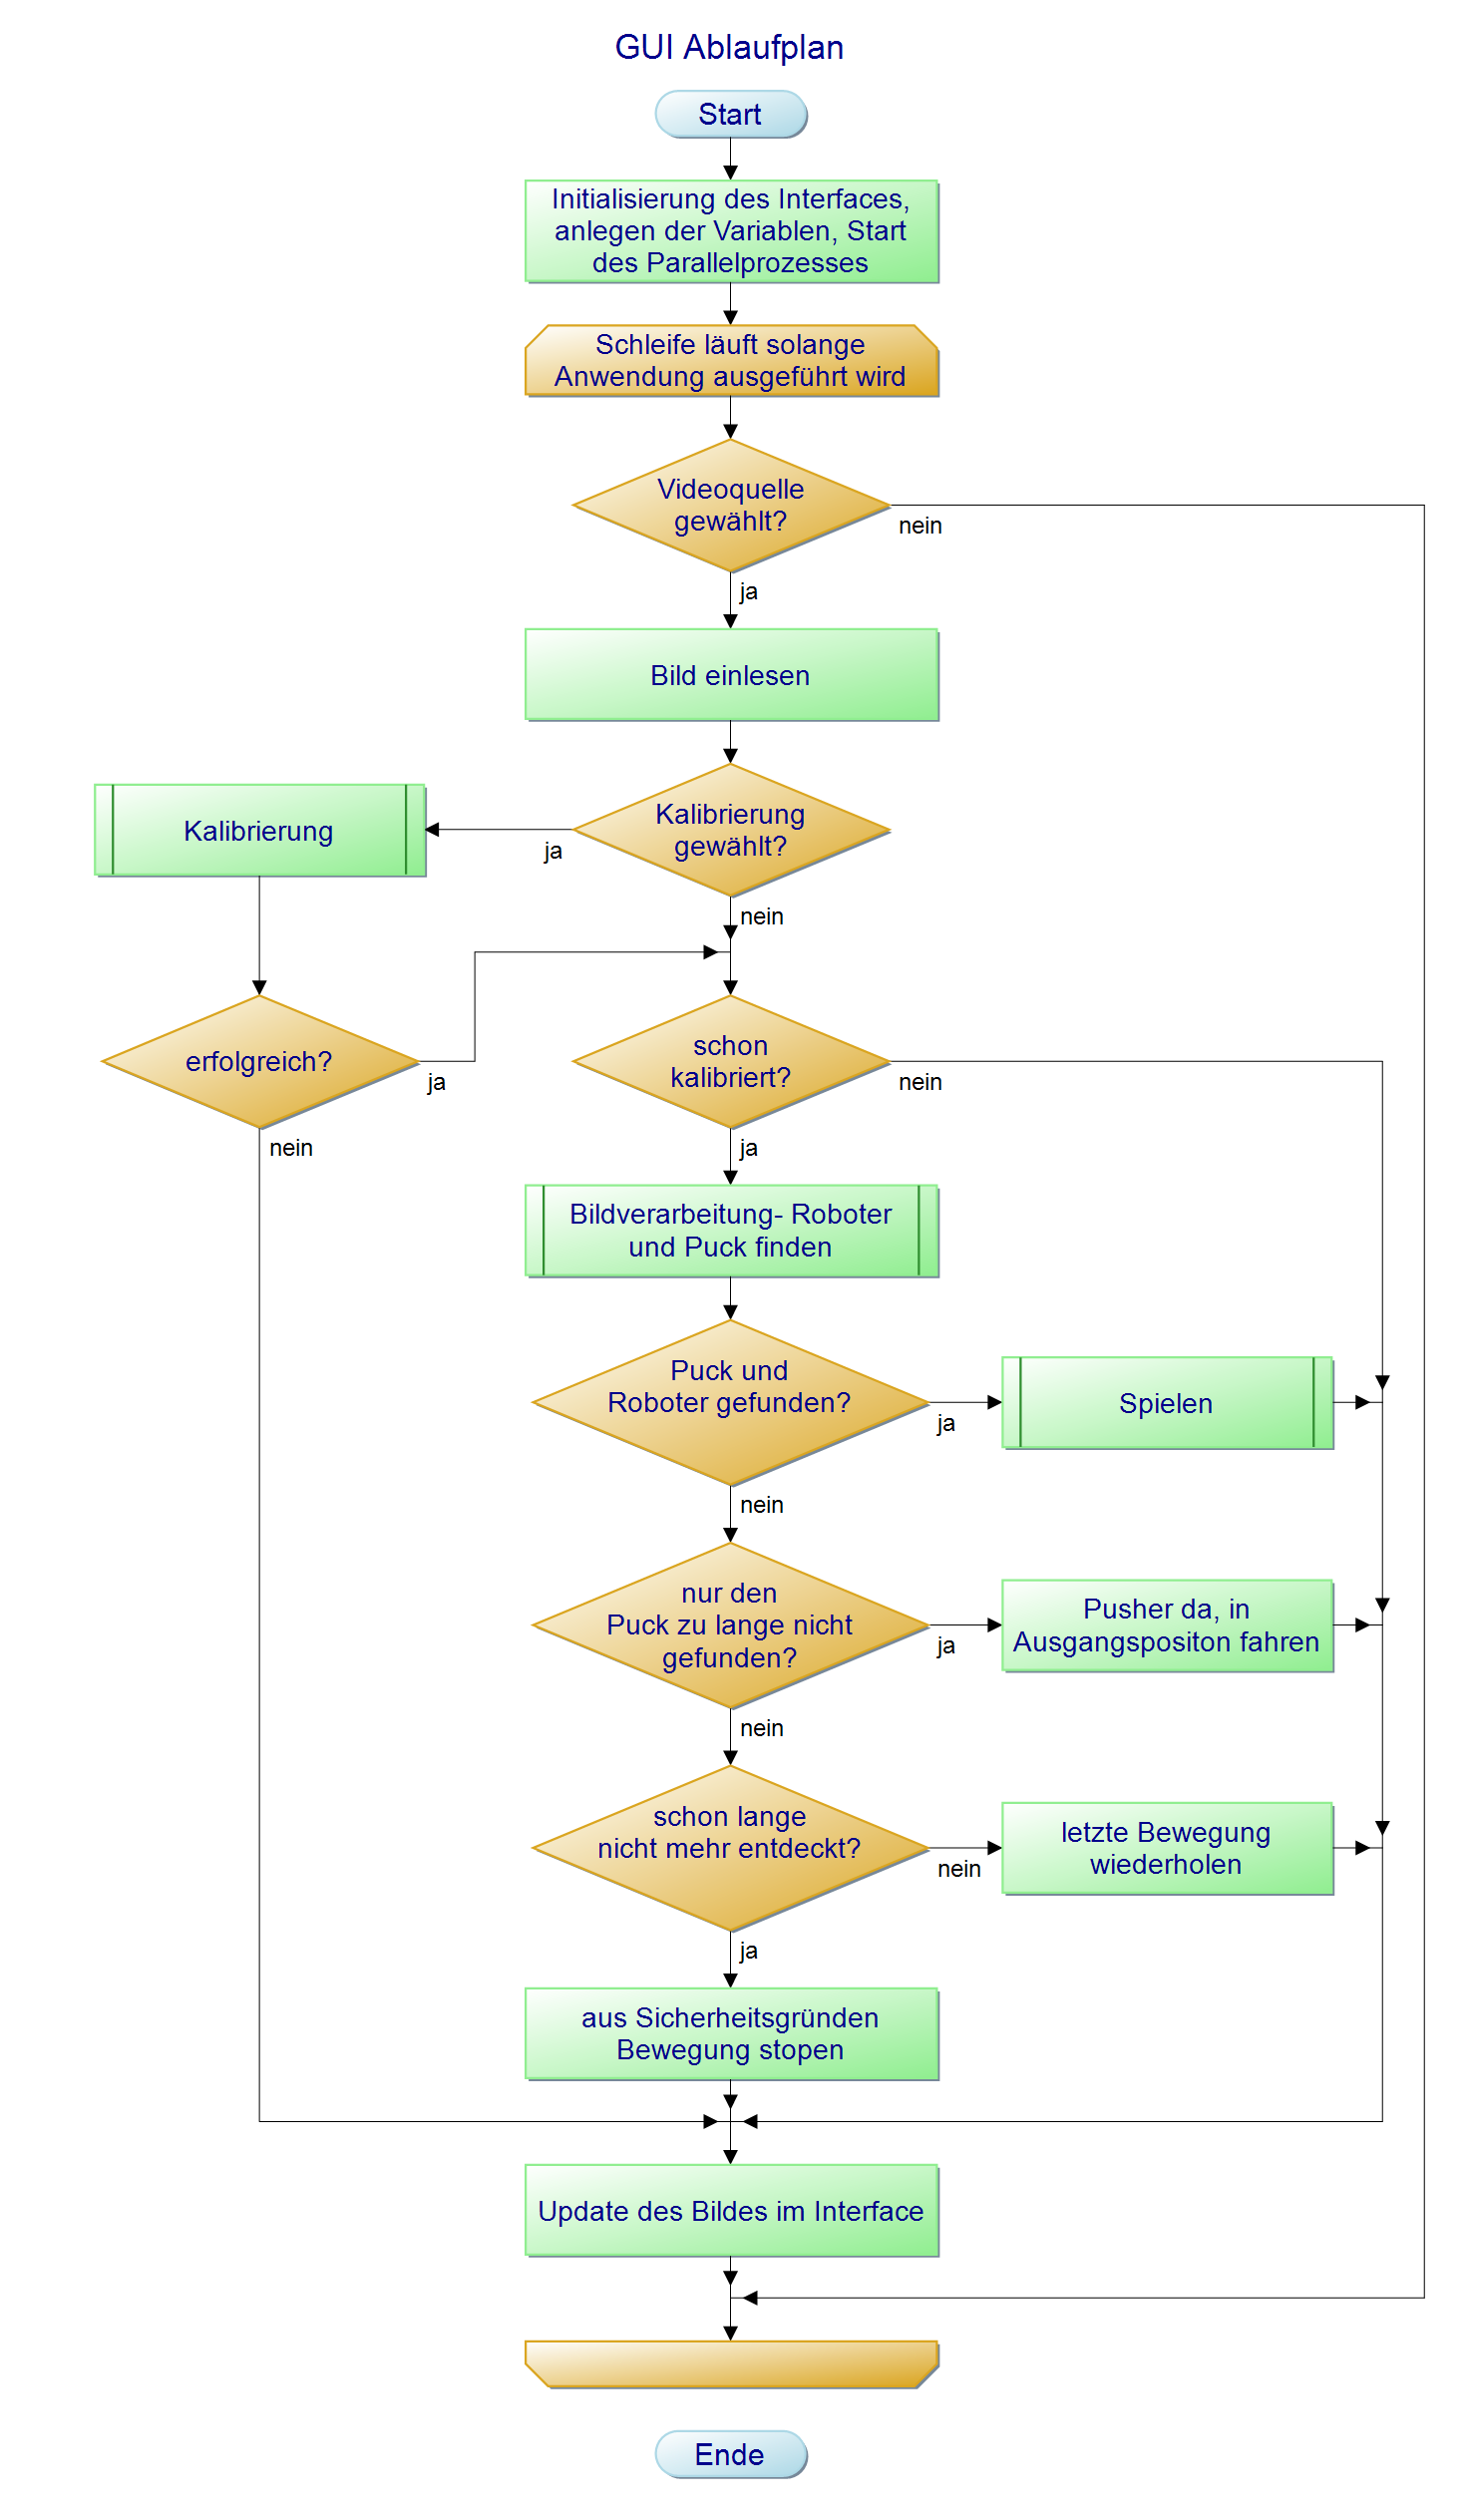
\includegraphics[scale =0.3]{images/gui_pap}
 \caption{Programmablaufplan des Standartablaufes}
 \label{gui_pap}

\end{figure}

\clearpage


\section{Kalibrierung}
\label{sect:kalib}
Bei der Kalibrierung geht es darum das Spielfeld vor der Kamera zu vermessen und auf das Spielfeld in der Unity Umgebung zu Übertragen. Das ist wichtig, da der Agent in der Softwareumgebung traininiert wurde und dem entsprechend auch Größen in Unity Längeneinheiten angegeben werden müssen. Angaben in Metern oder Pixeln müssen also umgerechnet werden. Da wir davon ausgehen können, dass die Kamera senkrecht über dem Spielfeld hängt und andere Verzerrungseffekte vernachlässigbar sind, können wir das Problem zweidimensional betrachten. Das bedeutet, dass die Felder zueinander verdreht um die Z-Achse, verschoben um die X- und Y-Achse und scaliert entlang der X- und Y-Achse sind. Eine Verkippung um die X- und Y-Achsen sowie eine Verschiebung in Z-Richtung fallen weg. \\
Um all diese Parameter berechnen zu können müssen auf dem realen Spielfeld mindestens drei Punkte ihrem Gegenstück aus der Unity Version zugeordnet werden.\\
Als markante Punkte haben wir die vier roten Kreise auf dem Spielfeld gewählt. Um diese auf dem Kamerabild zu erfassen muss zuerst ein bestimmter Farbberich extrahiert werden.Dazu wird das Ausgangsbild in den HSV-Farbraum überführt. Statt der Farbwerte für die Kanäle rot grün und blau sind Farben nun in durch die Kategorien Hue (Farbwert), Saturation (Reinheit, Sattigkeit), und Value (Helligkeit) beschrieben. Da eine Verstärkung der Beleuchtung nun nur noch eine Änderung am V-Wert (Value) zur Folge hat wird die Seperation eines Objekts dadurch viel stabiler.\\

\begin{figure} [h]
\begin{minipage}[t]{0.5\textwidth}
\vspace{0pt}

Nachdem der gewünschte vordefinierte Farbraum herausgefiltert wurde bleibt ein Binärbild, in dem alle Pixel die im Orginalbild in den Farbraum fallen, weiß sind. Mit hilfe der in OpenCV implementierten HoughCircles Funktion \cite{rhody2005lecture} können nun die Mittelpunkte der Kreise bestimmt werden. Dazu ist von Vorteil, dass die Größe vorher schon relativ genau bekannt ist. \\ 
Die Mittelpunkte werden danach mit vorher festgelegten Berichen abgeglichen. Da die Kamera fest moniert ist sollte nun klar sein, ob ein Kreis links oben, rechts oben, links unten oder rechts unten ist. Gibt es midestens drei Übereinstimmungen kann der Mittelpunkt des Spielfeldes und die Ausrichtung sowie die Skalierung relativ zum Unityfeld ermittelt werden. Mit diesem Wissen kann nun mittels zweier Funktionen die Umrechnung von realen in Unitykoordinaten und umgekehrt durchgeführt werden.\\
 Im Vergleich zum Programmablaufplan in der Abbildung \ref{gui_pap} ist der aus Abbildung \ref{kalib_pap} deutlich überschaubarer. Er ist bis auf eine Verzweigung geradlinig.
\end{minipage}
\hspace{0.1\textwidth}
\begin{minipage}[t]{0.3\textwidth}
\vspace{0pt}
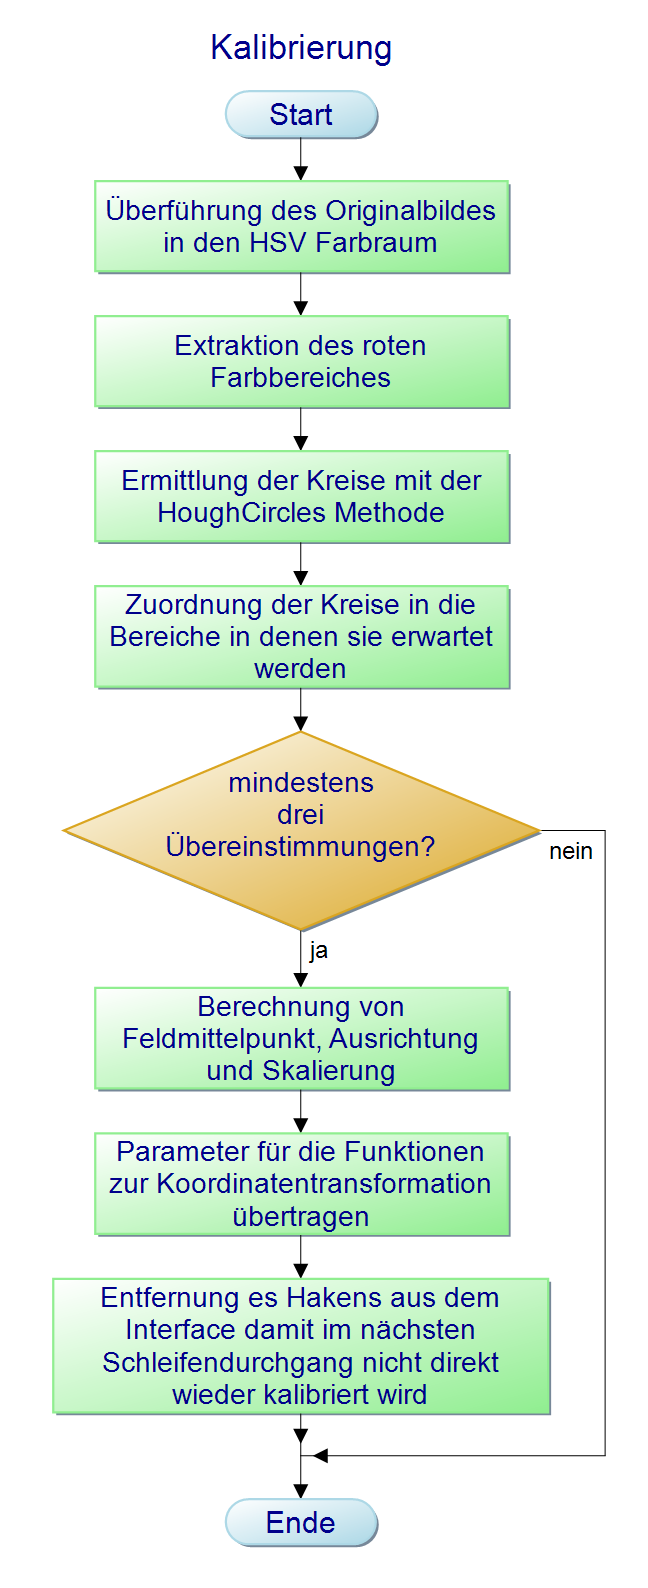
\includegraphics[scale =0.3]{images/kalibrierung_pap}
 \caption{Programmablaufplan der Kalibrierung}
 \label{kalib_pap}
\end{minipage}
\end{figure}

\begin{figure} [h]
\begin{minipage}[t]{0.4\textwidth}
\vspace{0pt}
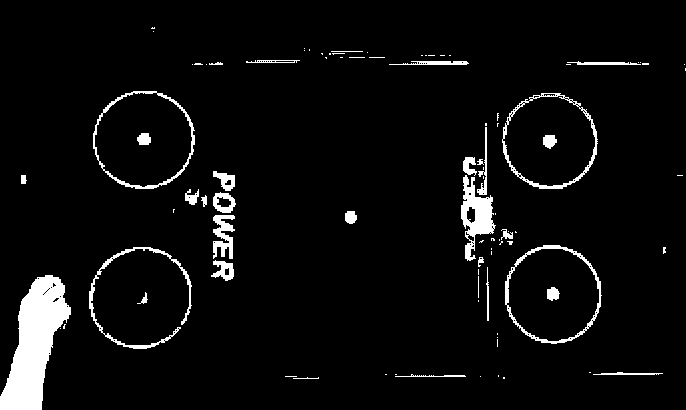
\includegraphics[scale =0.3]{images/kalib_bin}


\end{minipage}
\hspace{0.1\textwidth}
\begin{minipage}[t]{0.4\textwidth}
\vspace{0pt}
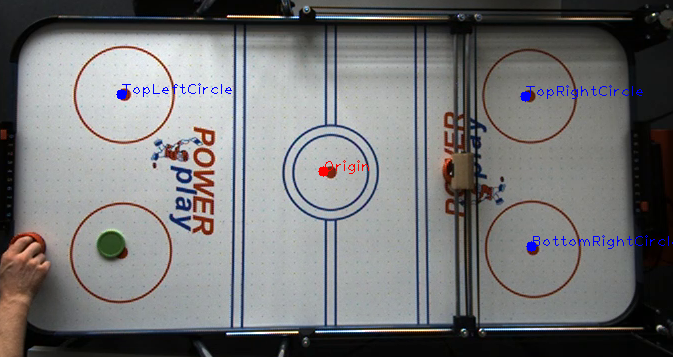
\includegraphics[scale =0.3]{images/kalib_circ}

\end{minipage}
 \caption{Zwischenergebnisse der Kalibrierung}
 \label{kalib_process}
\vspace{5pt}

Das linke Bild das Binärbild, das entsteht wenn nur ein bestimmter Farbbereich gewählt wird. Neben den Kreisen wird auch ein Teil der Schrift und der Arm des menschlichen Spielers mit binarisiert. Nach der HoughCircles Methode und der Zuordnung kann der Mittelpunkt des Spielfelds, wie man auf der rechten Seite erkennen kann ziemlich gut ermittelt werden.
\end{figure}

\clearpage
\section{Puck und Robotererkennung}
\label{sect:puck_robo_erk}
Um am realen Demonstrator den Agenten aus der Simulation nutzen zu können müssen alle Eingabewerte die während des Trainings von Unity bereitgestellt wurden hier anders ermittelt werden. Da viele Sensoren teuer und aufwändig zu implementieren sind haben wir uns entschlossen alle Daten aus den Kamerabildern zu beziehen. Die benötigten Daten sind Position des Pucks, Geschwindigkeit des Pucks und Position des Roboters. Alle drei Daten sind als X- und Y-Wertepaar nötig. Wie diese Imformationen erlangt werden soll in den folgen Abschnitten klar werden.\\


\begin{figure} [h]
\begin{minipage}[t]{0.35\textwidth}
\vspace{0pt}
Grundlage der Bildverarbeitung ist auch hier die Extaktion bestimmter Farbbereiche. Zuerst wird dazu wieder in den HSV- Raum übergegangen um dann ein Binärbild mit den erwünschten Bereichen in weiß zu erhalten. Da hier nicht mit der HoughCircles Funktion schnell ein Ergebniss erreicht werden kann wir danach eine kleine Errosion durchgeführt um das Binärbild übersichtlicher zu machen. Nach dieser Errosion sollten kaum mehr weiße Flecken außer der gewünschten Kontur übrig sein. Aus den verbleibenden Konturen wird dann die größte herausgesucht. Passt ihre Größe zu der des gesuchte Objekts (Puck oder Roboter) wird ihre Positon ermittelt. Hierzu werden die vorkalibrierten Funktionen verwendet. Im Unity Koordinatensystem sind die Werte dann geeignet für den Agenten. Aus der aktuellen Position, der letzen Position und der verstrichenen Zeit wird dann noch die Geschwindigkeit berechnent. 

\end{minipage}
\hspace{0.1\textwidth}
\begin{minipage}[t]{0.45\textwidth}
\vspace{0pt}
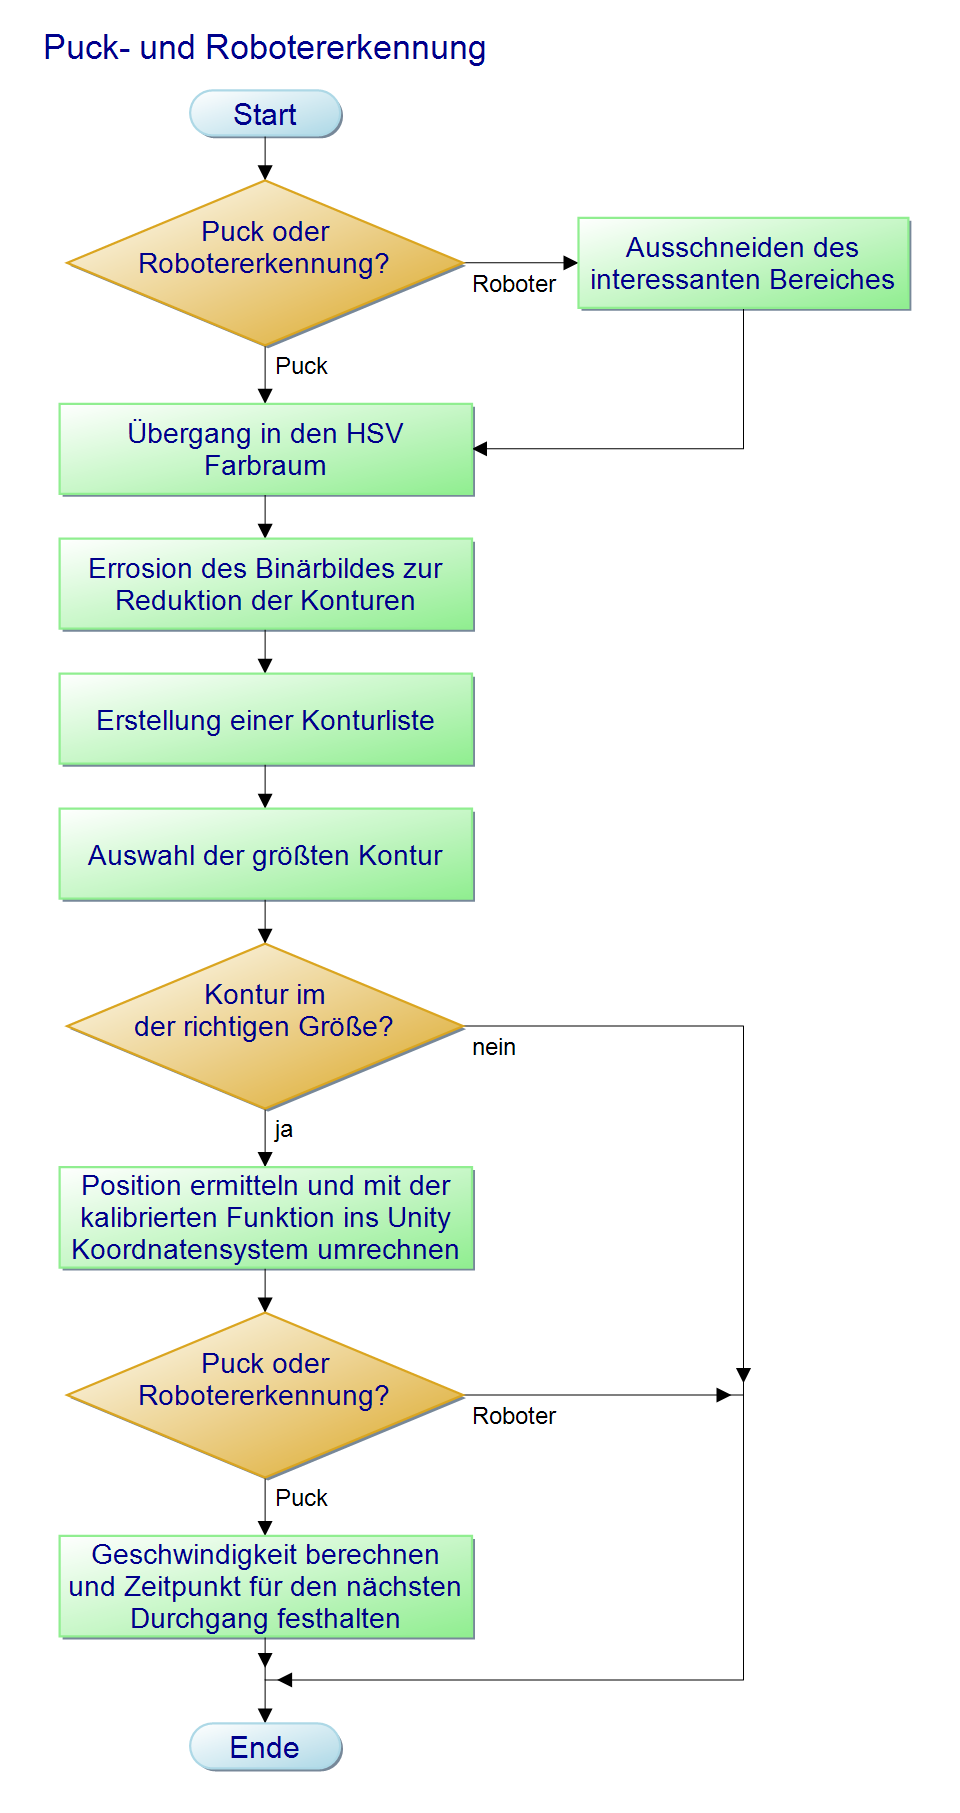
\includegraphics[scale =0.3]{images/bv_pap}
 \caption{Programmablaufplan der Puck- und Robotererkennung}
 \label{bv_pap}
\end{minipage}
\end{figure}

Der Vorgang ist bei Puck und Roboter vergleichbar. Die Hauptunterschiede sind die unterschiedlichen Farbräume, der Roboter kann sich nur in seiner Hälfte aufahlten und die Geschwindigkeit ist nur für den Puck zu berechnen. Zwar gibt es noch weitere kleine Unterschiede, beispielsweise bei der Errosion, aber bei beiden Erkennungen wird nach dem gleichen Plan verfahren.

\begin{figure} [h]
\begin{minipage}[t]{0.25\textwidth}
\vspace{0pt}

\includegraphics[scale =0.45]{images/bin_puck}
\end{minipage}
\hspace{0.05\textwidth}
\begin{minipage}[t]{0.25\textwidth}
\vspace{0pt}
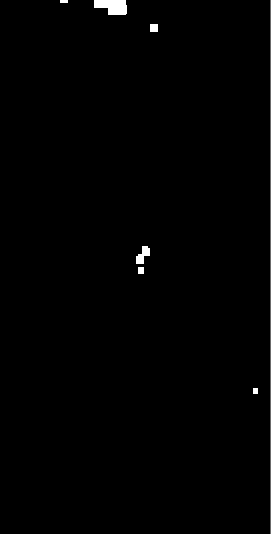
\includegraphics[scale =0.45]{images/bin_robo}
\end{minipage}
\hspace{0.05\textwidth}
\begin{minipage}[t]{0.25\textwidth}
\vspace{0pt}
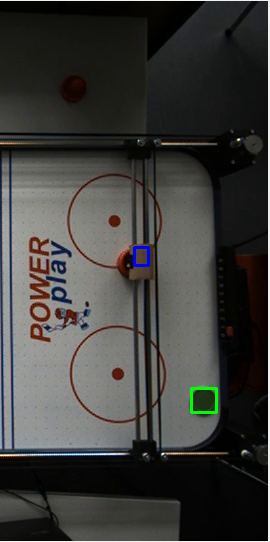
\includegraphics[scale =0.45]{images/detect}
\end{minipage}

 \caption{Zwischenergebnisse der Puck- und Robotererkennung}
 \label{bv_process}
\vspace{5pt}
In der Abbildung \ref{bv_process} ist dreimal der gleiche Feldabschnitt zu sehen. Links ist das errodierte Binärbild aus der Puckerkennung. Hier ist die Kontur des Pucks eindeutig zu erkennen. In der Mitte ist das errodierte Binärbild aus der Robotererkennung zu sehen. Durch schlechte Lichtverhältnisse und eine schlechte Farbwahl für den Roboter ist das Binärbild nicht besonders gut. Da jedoch der Bereich in dem sich der Roboter befinden kann bekannt ist kann die größte Kontur am oberen Bildrand ausgeschlossen werden. Der rechte Teil der Abbildung zeigt, dass Puck und Roboter richtig erkannt wurden.
\end{figure}

\clearpage
\section{Spielverhalten}
\label{sect:verh}
Dieser Abschnitt soll kurz darstellen wie sich der reale Demonstrator im Vergleich zu seinem digtalen Zwilling verhalten hat.\\
Ein großes Problem ist durch die Plattenbeschaffenheit aufgetretten. Die Platte ist nicht ganz eben. Dadurch fängt der Puck an manchen Stellen ohne Kontakt an zu gleiten. Solange der Puck schnell unterwegs ist, ist die Ablenkung durch die Unebenheit vernachlässigbar. Ein weiteres Problem das von der Plattenkrümmung her rührt, ist das der Roboter sich an manchen Stellen einklemmen kann. Da die Linerfühungen den Roboter auf einer Ebene führen ändert sich also der Abstand zwischen Tischplatte und Führung. Besonders am Rand und in den Ecken kann es deshalb zum stecken bleiben führen. Manchmal kann sich der Roboter unter Quietschen, Rattern und Schrittverlust an den Motoren wieder befreien aber selbst dieser Fall ist höchst unerfreulich. An besonders niedrigen Stellen kann es dagegen dazu kommen, dass sich der Puck zwischen Tischplatte und Roboter klemmt auch hier ist ein Spielabbruch meist die einzige vernünftige Lösung.\\
Neben den Defiziten, die durch die Hardware auftretten kommen noch andere dazu. Der Roboter kann bei weitem nicht die Bildwiederholungsrate, die im Interface angezeigt wird auf den Tisch bringen. Ein Teil des Zeitverlustes kommt von der Puck- und Robotererkennung. Ein weiterer Teil tritt bei der Kommunikation mit dem Arduino auf. Dadurch ist die Bewegung deutlich ruckeliger als es zu erwarten war. Das es einen kontinuierlichen Actionspace gibt, in dem alle möglichen Aktionen, mit Außnahme von Stehenbleiben, Vollgas sind verbesset die Situation nicht besonders.\\
Insgesamt ist die Leistung am Tisch unbrauchbar. Verglichen mit dem Spiel in Unity, dass fast nicht zu gewinnen ist, ist dieses Ergebnis noch nicht für eine Demonstration geeignet.


% --- Bibliography ---
\bibliography{bibfile} 
\bibliographystyle{ieeetr}


\end{document}